\documentclass[sigconf,natbib=true,anonymous=true]{acmart}
% \documentclass[manuscript,screen,review]{acmart}

% Needed to fix an acmart problem with line numbering. AFAICT line 
% numbers are not expected in sigconf, so it should be a no-op.
\makeatletter
\providecommand{\@LN}[2]{}
\makeatother

% % Fonts used in the template cannot be substituted; margin 
% % adjustments are not allowed.
% %
% % \BibTeX command to typeset BibTeX logo in the docs
% \AtBeginDocument{%
%   \providecommand\BibTeX{{%
%     \normalfont B\kern-0.5em{\scshape i\kern-0.25em b}\kern-0.8em\TeX}}}

%% Rights management information.  This information is sent to you
%% when you complete the rights form.  These commands have SAMPLE
%% values in them; it is your responsibility as an author to replace
%% the commands and values with those provided to you when you
%% complete the rights form.
\setcopyright{acmcopyright}
\copyrightyear{2022}
\acmYear{2022}
\acmDOI{XXXXXXX.XXXXXXX}

%% These commands are for a PROCEEDINGS abstract or paper.
\acmConference[SIGIR '22]{Make sure to enter the correct
  conference title from your rights confirmation email}{June 03--05,
  2022}{Madrid, Spain}
%
%  Uncomment \acmBooktitle if the title of the proceedings is different
%  from ``Proceedings of ...''!
%
\acmBooktitle{SIGIR '22: Proceedings of the 45th International ACM SIGIR Conference on Research and Development in Information Retrieval,
 July 11--15, 2022, Madrid, Spain} 
% \acmPrice{15.00}
% \acmISBN{978-1-4503-XXXX-X/18/06}

%
% Submission ID.
% Use this when submitting an article to a sponsored event. You'll
% receive a unique submission ID from the organizers
% of the event, and this ID should be used as the parameter to this command.
% \acmSubmissionID{123-A56-BU3}

%
% The majority of ACM publications use numbered citations and
% references.  The command \citestyle{authoryear} switches to the
% "author year" style.
%
% If you are preparing content for an event
% sponsored by ACM SIGGRAPH, you must use the "author year" style of
% citations and references.
% Uncommenting
% the next command will enable that style.
%\citestyle{acmauthoryear}

%% The "author" command and its associated commands are used to define
%% the authors and their affiliations.
%% Of note is the shared affiliation of the first two authors, and the
%% "authornote" and "authornotemark" commands
%% used to denote shared contribution to the research.
\author{Ben Trovato}
\authornote{Both authors contributed equally to this research.}
\email{trovato@corporation.com}
\orcid{1234-5678-9012}
\author{G.K.M. Tobin}
\authornotemark[1]
\email{webmaster@marysville-ohio.com}
\affiliation{%
  \institution{Institute for Clarity in Documentation}
  \streetaddress{P.O. Box 1212}
  \city{Dublin}
  \state{Ohio}
  \country{USA}
  \postcode{43017-6221}
}

\author{Lars Th{\o}rv{\"a}ld}
\affiliation{%
  \institution{The Th{\o}rv{\"a}ld Group}
  \streetaddress{1 Th{\o}rv{\"a}ld Circle}
  \city{Hekla}
  \country{Iceland}}
\email{larst@affiliation.org}

\author{Valerie B\'eranger}
\affiliation{%
  \institution{Inria Paris-Rocquencourt}
  \city{Rocquencourt}
  \country{France}
}

\author{Aparna Patel}
\affiliation{%
 \institution{Rajiv Gandhi University}
 \streetaddress{Rono-Hills}
 \city{Doimukh}
 \state{Arunachal Pradesh}
 \country{India}}

\author{Huifen Chan}
\affiliation{%
  \institution{Tsinghua University}
  \streetaddress{30 Shuangqing Rd}
  \city{Haidian Qu}
  \state{Beijing Shi}
  \country{China}}

\author{Charles Palmer}
\affiliation{%
  \institution{Palmer Research Laboratories}
  \streetaddress{8600 Datapoint Drive}
  \city{San Antonio}
  \state{Texas}
  \country{USA}
  \postcode{78229}}
\email{cpalmer@prl.com}

\author{John Smith}
\affiliation{%
  \institution{The Th{\o}rv{\"a}ld Group}
  \streetaddress{1 Th{\o}rv{\"a}ld Circle}
  \city{Hekla}
  \country{Iceland}}
\email{jsmith@affiliation.org}

\author{Julius P. Kumquat}
\affiliation{%
  \institution{The Kumquat Consortium}
  \city{New York}
  \country{USA}}
\email{jpkumquat@consortium.net}

%%%%%%%%%%%%%%%%%%%%
%%%%%%%%%%%%%%%%%%%%
% EDITING LINK: 
% https://www.overleaf.com/3575751412sjsdmszkxsyh
%%%%%%%%%%%%%%%%%%%%
%%%%%%%%%%%%%%%%%%%%

% \usepackage{soul} %% Soul does not play well with acmart
\usepackage{url}
% % \usepackage[hidelinks]{hyperref}https://www.overleaf.com/project/614b5cc61d38655dce466002
% \usepackage[small]{caption}
\usepackage{graphicx}
\usepackage{amsthm}
\usepackage{booktabs}
\usepackage{algorithm}
\usepackage{algorithmic}
\usepackage{cleveref}
\usepackage{lipsum}

\urlstyle{same}

% % =======================================
% % my imported packages

\usepackage{amsmath}
\usepackage{bm}
% \usepackage{amssymb}          % duplicates something in acmart
\usepackage{listings}
% \usepackage[ruled,vlined]{algorithm2e}
\include{pythonlisting}

\newcommand{\pseudosection}[1]{\vspace{1.5ex}\noindent \textit{{#1:~~}}}
% \newcommand{\pseudosection}[1]\indent{{{}}}

\usepackage{todonotes}
\newcommand{\todokdinline}[1]{\todo[color=red!20,inline]{{KD: \small #1}}}
\newcommand{\todokd}[1]{\todo[color=red!20]{{\small #1 -- Kasra}}}
% \newcommand{\todocainline}[1]{\todo[color=yellow!20,inline]{{CA: \small #1}}}
\newcommand{\todocm}[1]{\todo[color=green!40]{\small #1 -- Cynthia}}
\newcommand{\todocmi}[1]{\todo[inline,color=green!40]{\small #1 -- Cynthia}}
\newcommand{\todoff}[1]{\todo[color=blue!20]{\small #1 -- Frank}}
\newcommand{\todoed}[1]{\todo[color=cyan!20]{\small #1 -- Ed}}

\newcommand{\CitationNeeded}[1]{{\textbf {\color{red}Cite #1}}}
\newcommand{\ProofRead}[1]{{\textbf {\color{red}Proofread please #1}}}
\newcommand{\Complete}[0]{{\textbf {\color{red}Complete it }}}
\newcommand{\Rephrase}[1]{{\textbf {\color{red}Rephrase please #1}}}

% \newcommand{\citet}[1]{\cite{#1}} % This is used because \citet didn't work with their author kit % It does now

% =======================================
\title{Multimodal Contrastive Learning for Object Retrieval in the Face of Modality Failures}

\begin{document}

% Todo list
% \begin{enumerate}
%     \item \st{Lit search}
% \end{enumerate}
% \newpage

% ***************** The BEGINNING of the paper *****************

\begin{abstract}
    % Grounded language understanding, in which natural language is used as a query against objects in a physical environment, allows a real-world, intuitive mechanism by which users can instruct physical agents to engage in tasks such as object retrieval. Visuolinguistic approaches to such object inference tasks typically involve training on large pools of image/text pairs and then using language to subselect elements of the sensed environment. However, physical agents such as robots typically have access to sensory and interactive modalities beyond vision, and learning from multiple modalities can improve performance on downstream tasks. In order to fully leverage multimodal training data while being robust to missing information, we propose a generalized distance-based loss function that can be extended to learn retrieval models that incorporate an arbitrary number of modalities. We demonstrate the usability of our model on a grounded language object retrieval scenario, where an intelligent agent has to select an object given an unconstrained language command. We leverage four modalities including vision, depth sensing, text, and speech, and we show that our model can outperform state-of-the-art contrastive models when modalities are ablated.

    % shorter version
    
    We propose a generalized distance-based loss function that can be used to learn retrieval models that incorporate an arbitrary number of views of a particular piece of data, and compounded by the challenge of retrieval when a modality becomes unavailable. 
    Our study is motivated by needs in robotics and computer-human interaction, where an agent has many sensors and thus modalities in which a human may interact: voice, text, images, and depth, both to communicate a desired goal and for the agent to recognize a desired target object. 
    Tying these various modalities together relates to the task of grounded language understanding, in which natural language is used as a query against objects in a physical environment, allowing a real-world, intuitive mechanism by which users can instruct physical agents to engage in tasks such as object retrieval.
    However, current work has neglected the real-world constraint that sensors fail: hardware can become damaged or shipped with defects, sensors can get blocked or obstructed, and various adverse but not uncommon conditions that remove a modality from use. For practical applications, we need mechanisms for accurate object retrieval given that a modality may fail without notice. 
    We demonstrate the usability of our model on a grounded language object retrieval scenario, where an intelligent agent has to select an object given an unconstrained language command. We leverage four modalities including vision, depth sensing, text, and speech, and we show that our model can outperform state-of-the-art contrastive models when modalities are ablated.
\end{abstract}

\settopmatter{printfolios=true} % Page numbers please 
% 9 pages without references.

% \begin{enumerate}
%     \item Objects of five things we select from
%     \item \textcolor{green}{DONE} Adding an overview of the whole process 
%     \item \textcolor{blue}{PROG} Go into more details in section 4 and give examples 
%     \item Move images around
%     \item Quant result section is not complete
%     \item \textcolor{green}{DONE} put the graphs in modality ablation or merge quant and qual
%     \item \textcolor{green}{DONE} add dropping R D graphs
%     \item A paragraph in related work about grounded language 
%     % \item Don't mess with additional experiments
% \end{enumerate}
%===================================================================

\maketitle
% \setcounter{page}{1}

%===================================================================

% \section{SIGIR Papers}
% \begin{enumerate}
%     \item \href{https://dl.acm.org/doi/pdf/10.1145/3397271.3401430}{FashionBERT}
%     \item \href{https://dl.acm.org/doi/pdf/10.1145/3397271.3401265?casa_token=W8NqNWp0UQkAAAAA:w-iRUnNhmytDKCUiYzaUPG0bI_yyo8Bzxwro_eOC-zl5VDIGRVT2dvixvnCwLJ0iEKqYo1LkQIWXVA}{CrossBERT}
    
% \end{enumerate}

\section{Introduction}
\label{intro}

Humans use multiple sensory inputs to understand, interact with, and retrieve information from the world around them. It is intuitive that agents learning about the world, upon encountering new concepts and new objects, should form a model that incorporates information from all available sensors and data sources. 
% 
Grounded language understanding, in which natural language is used as a query against objects in a physical environment, allows a real-world, intuitive mechanism by which users can instruct physical agents to engage in tasks such as object retrieval. Visuolinguistic approaches to such object inference tasks typically involve training on large pools of image/text pairs and then using language to subselect elements of the sensed environment~\cite{hong2021gilbert}. Although physical agents such as robots typically have access to sensory and interactive modalities beyond vision, and learning from multiple modalities can improve performance on downstream tasks, most approaches use at most two sensory inputs (e.g., visual data such as RGB images) with single labels, such as those provided by textual natural language. Simultaneously using additional inputs from different modalities is an underexplored area, in part due to the domain-specific nature of such \textit{n}-ary learning approaches. With the modern proliferation of audio and text based communication and proliferation of home agents (e.g., iRobot vacuums and Alexa/Google Home), there is a growing need to handle more modalities, and simultaneously their potential failures. 

One difficulty with working with complex multimodal data is the increased likelihood that one or more modalities may have missing information. Current multimodal approaches are typically not robust to the loss of one or more modalities at test time, as may happen if, for example, a physical agent fails to retrieve data from a particular sensor. In order to fully leverage multimodal training data while being robust to missing information, we propose a generalized distance-based loss function that can be extended to learn retrieval models that incorporate an arbitrary number of modalities.

We consider the domain of grounded language-based object retrieval~\cite{hu2016natural, triplet_loss_2021_CVPR}, in which objects in an environment must be identified based on linguistic instructions. This can be considered a special case of image retrieval~\cite{huang2017deep, ma2020large, novak2015large, vo2019composing} in which objects are identified using visual inputs in combination with other sensor modalities. Approaches to acquiring grounded language have explored various combinations of sensor inputs such as depth and RGB with labels provided by textual language or  speech~\cite{RichardsDarvishMatuszekCategoryFree20}. 
However, despite the multisensory nature of object retrieval, much of the existing work has not previously been extended to include an arbitrary number of modalities. 

The high level goal of this work is to take arbitrary input modalities about novel objects, including both spoken and written language, and build a model that allows a system to correctly retrieve that object given a subset of those input modalities. This is a generalization of approaches to grounded language learning in which specific input modalities are labeled with language to allow for future identification, but explicitly seeks to be agnostic about the nature of the individual sensory and linguistic inputs. Our contributions are as follows:
\begin{enumerate}
    \item Proposing a general distance-based loss function formulation for multimodal learning that can be extended to an arbitrary number of modalities.
    \item Outperforming state-of-the-art contrastive learning models when one or more modalities are ablated at test time, demonstrating robustness in the face of missing information.
    % \item Outperforming state-of-the-art models for grounded language learning by differentiating visual input modalities such as RGB and depth, rather than combining them into a single modality.
    \item Demonstrating the separate utility of speech and text as sources of label information by treating them as sensory input modalities, rather than explicitly as labels.
\end{enumerate}

The remainder of this paper is organized as follows. In \cref{sec:Related-Work}, we describe existing work on visuolinguistic retrieval, contrastive learning, and multimodal learning. In \cref{sec:Problem-Description}, we formalize the object retrieval problem and give examples of the data under consideration. In \cref{sec:Method}, we describe our novel approach to learning models of linguistically-driven queries against a multimodal set of objects. Finally, in \cref{sec:Experiments}, we demonstrate the effectiveness of our approach against traditional contrastive learning and supervised contrastive learning baselines, both for the general learning problem and in the case of missing information at test time.

% \todocmi{NOTES: Some things are probably less informative or more ambiguous (e.g., depth for differentiating round things). So instead of predicting a single vector output, predict a vector and a covariance that captures uncertainty; could potentially use that to do more accurate search, or to handle really uncertain modalities (e.g., just drop speech when it's uninformative).} 

%===================================================================

\section{Related Work}
\label{sec:Related-Work}

There is extensive work on the task of image retrieval, of which physical object retrieval can be considered a special case. In this task, language is used to formulate queries against datasets of images, for example in text-and-image matching tasks for fashion data~\cite{gao2020fashionbert, wen2021comprehensive}, sketch retrieval~\cite{huang2017deep}, and general photographs of objects~\cite{ma2020large, novak2015large, hong2021gilbert}. Prior work has focused solely on language and visual modalities, using text or a combination of language and vision to perform visual retrieval~\cite{vo2019composing}. While recent works have focused on grounding with respect to a knowledge set \cite{10.1145/3357384.3357889,10.1145/3397271.3401097}, our work focuses on robust multimodal learning over to perform grounding over an arbitrary number of input modalities. 

The growing number of datasets that contain modalities beyond images and text demonstrates the importance and the challenge of this task. \citet{bagher-zadeh-etal-2018-multimodal} introduce a large dataset of multimodal opinion sentiment and emotion intensity (CMU-MOSEI) for sentiment analysis and emotion recognition. They also introduce a novel multimodal fusion technique called the Dynamic Fusion Graph (DFG).~\citet{GoLD_UMBC} present a multimodal dataset of household objects containing RGB images, depth images, written language, and spoken language, which has been used to support learning grounded language directly from speech given small datasets~\cite{KebeAAAI2022}. 
\citet{baltrusaitisMultimodalMachineLearning2019} propose a new taxonomy of multimodal machine learning by introducing five technical challenges in addition to typical early and late fusion categorization. They cover different approaches to multimodal machine learning such as \textit{representation}, \textit{translation}, \textit{alignment}, \textit{fusion}, and \textit{co-learning}. In this project, we focus on alignment, the process of identifying the direct relationship between elements across modalities.

We highlight a key difference with recent work like \citet{10.1145/3397271.3401232} and \citet{10.1145/3331184.3331213} who develop multi-modal retrieval models. These retrieval models are class based, where the model is trained to recognize any object of the same retrieval class as being ``same''. Our method and data is instance based, where different objects are not considered ``same'' even if they have the same class, due to the grounding goals of our work (i.e., the agent should identify the specified object, not equivalent objects). These works also do not consider the failure of a modality that is our target of interest. 

A number of different approaches have been proposed for linguistic-based alignment learning. \citet{alayrac2020self} use a self-supervised contrastive learning method to learn and combine representations from three modalities of visual, audio, and language. Audio and visual domains are mapped to the same space because they are fine-grained, containing dense information for each frame of video. These embeddings are then mapped to a coarse space where text is also mapped. Their network respects specificity and comparability of different modalities. The loss function they define consists of two distance-based terms for the corresponding spaces, differing from ours in that they do not handle arbitrarily many modalities and do not focus on robustness in the face of modality drop-outs. \citet{Nguyen-RSS-20} take a similar approach and perform pairwise cosine similarity to align images and natural language text descriptions to perform object retrieval tasks. \citet{triplet_loss_2021_CVPR} take a cross-modal manifold alignment approach to grounded language learning using triplet loss \cite{Chechik:2010:LSO:1756006.1756042}, and perform object retrieval by connecting text descriptions of objects to their corresponding RGB-D images.

Another related approach is contrastive learning~\cite{qin2021world}, which is based on the idea of similarity and distance of elements of training data~\cite{NEURIPS2020_supervised_contrastive,chen2020simple}. Triplet loss is also a special case of contrastive loss~\cite{NEURIPS2020_supervised_contrastive}. Contrastive loss is mostly used in self-supervised learning~\cite{bui2021self, alayrac2020self,chen2020simple}, with the exception of \citet{NEURIPS2020_supervised_contrastive}, who use contrastive loss for a supervised problem. Most of these methods are implemented for a non-multimodal dataset (e.g., RGB images only). Our work is a specialization of contrastive loss that is focused on the multimodal input and- language problem.

We note in particular that standard triplet learning approaches often require an expensive \textit{mining} step to find harder negative samples to enable effective learning \cite{Hoffer2015,Schroff2015,DBLP:conf/eccv/2018-9,DBLP:conf/eccv/ZhaoJQLH18,Zhai2018}. This is problematic from throughput and scalability, as run time becomes quadratic in batch size. Our approach does not require mining to obtain good performance, alleviating these issues along with their complicated history in reproducibility and parameter tuning \cite{Musgrave2020,Raff2020c,Raff2019_quantify_repro}. 

Some of the most closely related work focuses on learning based on more than two input modalities. \citet{Veit_2018_CVPR} train a joint model of images, hashtags, and users to perform image retrieval. Their task is similar to ours---given a description, we want to find the image/object in the scene that best matches the description. They tackle this problem by forming a three-way tensor product model. They use a ranking loss to train the model where the score of an observed triplet is higher than an unobserved triplet. They sample six negative triplets per positive sample triplet, and use each of them as a negative in the loss. The downstream retrieval task is then simply done by taking the argmax of the tensor product for a given user. This work differs from ours in that it becomes computationally complex as more and higher-dimensional modalities are added.

\citet{semihet_three_way_Lei_2020} use inputs from three modalities of image, sketch, and edgemap to perform image retrieval given the sketch. They use co-attention mechanism, and their loss function contains alignment loss, cross-entropy loss, and sketch-edgemap contrastive loss. \citet{Mittal2020M3ER} use Canonical Correlational Analysis (CCA) to differentiate between ineffective and effective modalities for the emotion recognition task from multiple input modalities including face, speech, and text. Multimodal learning has been used for different applications including but not limited to object retrieval. \citet{Deception_ICMI_2014} use language, physiological response, and thermal sensing to detect deceit. \citet{het_data_fusion_liu_IEEE_2017} take two modalities as input and output predictions in a third modality. \citet{tursun2021efficient} uses quadruplet loss for two modalities only; image and sketch. A quadruplet is composed of a sketch picture as an anchor, a negative example from sketch domain, a negative example from picture domain,  and a positive example from picture domain. \citet{chen2017beyond} also uses quadruplet loss, but does not support multiple domains. In contrast, our method is not restricted to two modalities.
% \todo[inline]{talk about CLIP and DALL-E here}

To the best of our knowledge, there has been limited work on incorporating more than three modalities into a general learning approach. Our proposed loss function closely resembles work on quadruplet loss~\cite{chen2017beyond,tursun2021efficient} but is intended to scale to an arbitrary number of modalities.

%===================================================================

\section{Problem Description}
\label{sec:Problem-Description}

Given a language command, for example either text or speech, that describes an object, we want our model to retrieve the correct object from a set of objects. This problem is an exemplar of tasks found in the area of grounded language learning in the fields of robotics and natural  language processing. Intuitively, the goal is to take unconstrained natural language queries and select the appropriate object based on the complete set of sensor inputs available to the agent. We demonstrate on a domain containing four modalities, all of which refer to objects in the environment: spoken language, written text, RGB (image) inputs, and depth camera inputs. \Cref{fig:experimental-setup} illustrates a small visualization of our object retrieval task: the spoken query ``A white textbook titled algorithms'' is provided to our contrastive model, which identifies the item (outlined in red, and represented by up to four different modalities) as the most likely item the query is referring to.

\begin{figure}[tb]
\centering
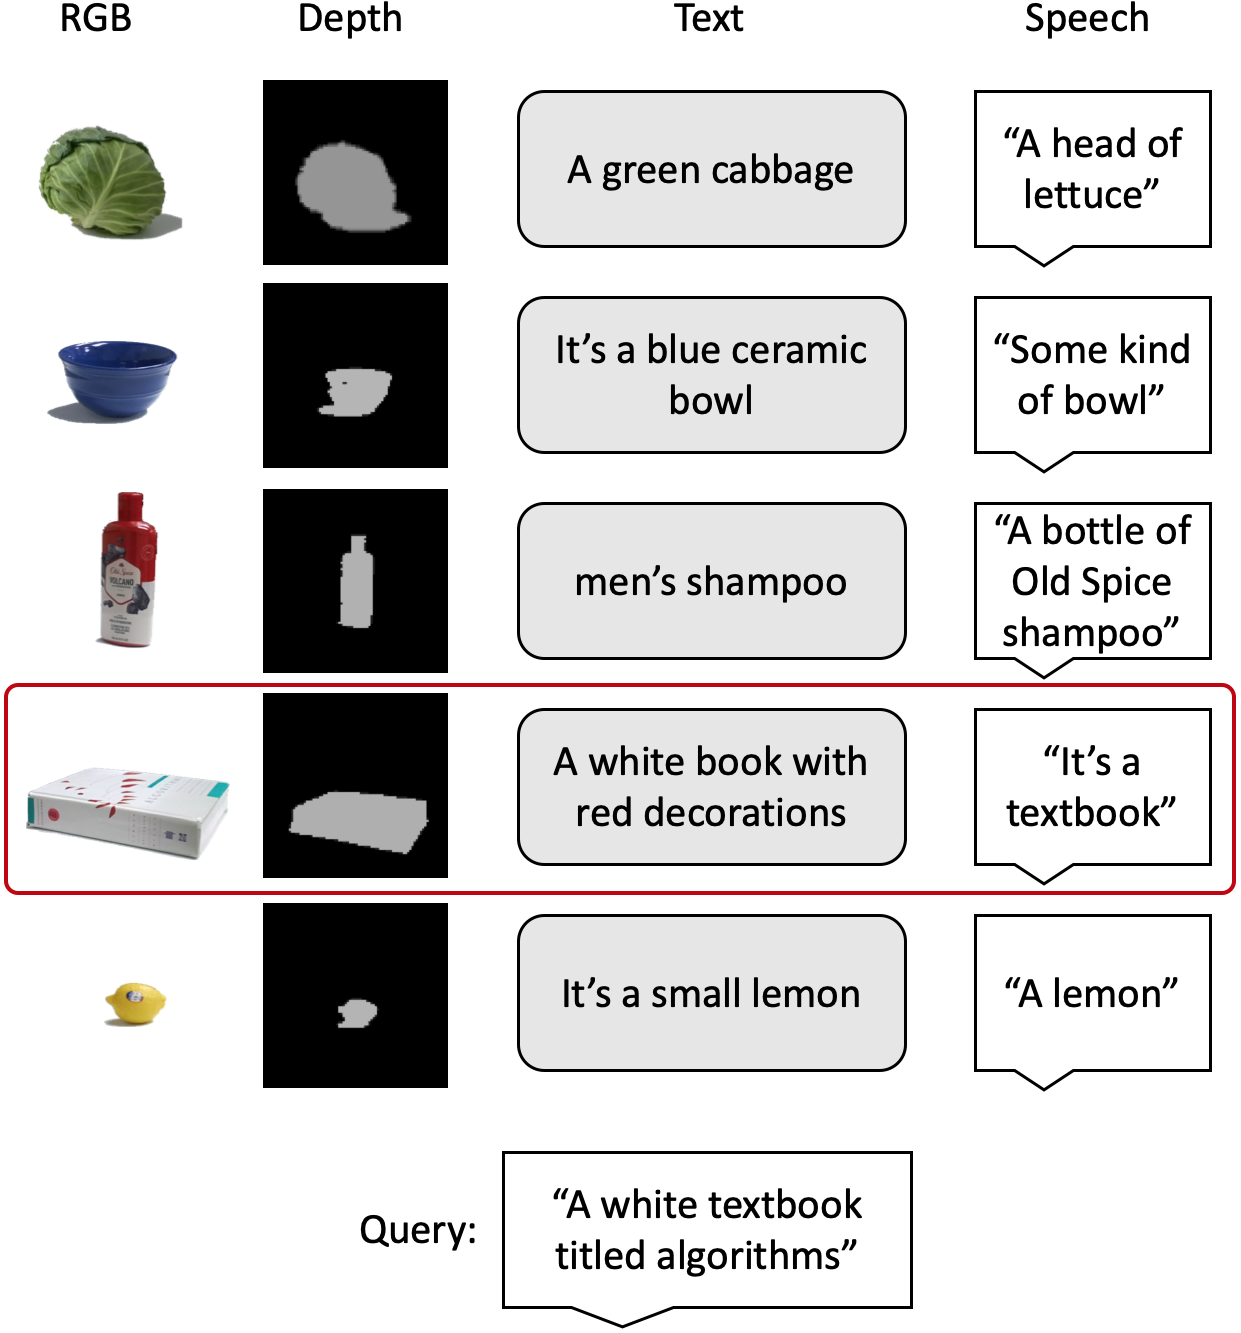
\includegraphics[width=.99\columnwidth]{Figures/experiment-setup.png}
\caption{
The experimental object retrieval setup, in which objects are represented by four modalities: an RGB image, a depth image, spoken descriptions, and textual descriptions. Given a query in some modality, our approach seeks to select the object that is the best fit, per a trained model. This approach, detailed in \cref{sec:Method}, is able to rank objects as to appropriateness even when one or more modalities is ablated at test time (e.g., textual descriptions are missing), and outperforms state-of-the-art contrastive learning approaches on this task.
}
\label{fig:experimental-setup}
\end{figure}

More formally, we consider a spoken language command $x_s$, a textual language command $x_t$, a set of RGB images $X_r = \{x_r^{(1..n)}\}$, and a set of depth images $X_d = \{x_d^{(1..n)}\}$, the task is to retrieve the correct object by choosing the index that has the minimum distance from either of the language commands across all modalities.
Depending on which modalities are or are not ablated, we consider up-to four distances: ``sr,'' a vector of distances between $x_s$ and all RGB images in $X_r$; ``sd,'' a vector of distances between $x_s$ and all depth images in $X_d$; ``tr,'' a vector of distances between $x_t$ and all RGB images in $X_r$; and ``td,'' a vector of distances between $x_t$ and all depth images in $X_d$. In order to select the correct object, we first perform a component-wise average of the relevant modality pair distances for the available modalities. Then, we select the object which had the minimum distance, i.e., we perform an argmin on this average vector of multiple-modality distances. Depending on the missing/available sensors during test time, we might have any combination of these four distances. For example, if no written instructions are available at test time,\footnote{This setting is particularly salient. While large bodies of text are frequently available at training time, a person interacting directly with a physical agent may well prefer to use spoken instructions.} we compute the component-wise average of $sr$ and $sd$, and then select the object whose coordinate resulted in the lowest average distance. This method allows us to extend our model to support arbitrary modalities while remaining robust to test cases in which some modalities are missing or incomplete. 


%===================================================================

\section{Approach}
\label{sec:Method}

In keeping with previous work on the closely related problem of image retrieval, we focus on contrastive loss approaches, in which the goal is to learn an embedding of data in which similar samples---in our case, samples belonging to the same class of object---are embedded `close' to one another, while dissimilar samples are farther apart. We develop a novel loss function that simultaneously minimizes intra-class distances and maximizes inter-class distances across each pair of modalities, yielding a model that is both effective at the retrieval task defined above and robust to modality dropouts at test time.

\subsection{Distance-based Loss}
\label{ssec:distanceloss}

For $M$ modalities, we define a distance-based loss function which can be used for arbitrary number of modalities. Our proposed method is an extension of the well-known similarity-based triplet loss~\cite{Carvalho-cooking-triplet,triplet_loss_2021_CVPR}, and is similar to contrastive loss~\cite{chen2020simple,NEURIPS2020_supervised_contrastive} under some settings.
Triplet loss-based learning works by forcing similar concepts from different domains `together' in some shared embedding space, while forcing dissimilar concepts `apart.' It is so named because it relies on three data points from the training set: a positive, a negative, and an anchor point. In our setting, the anchor and positive instances are from the same class, but in different modalities. 

However, standard triplet loss cannot be used for more than two modalities. Therefore, we extend this concept as follows. During training, we sample two sets of data points from each modality---one positive set (referring to a specific object) and one negative set (referring to some different object).
Unlike some prior triplet loss methods~\cite{GoLD_UMBC,triplet_loss_2021_CVPR}, the anchor is not randomly chosen from different modalities in each batch. Instead, we choose one \textit{domain} as an anchor (in our experiments, language). We consider the following formulation:

\begin{itemize}
    % \item data point: a row in the csv/tsv file.
    \item Positive (Instance): A set of embeddings of one data point (e.g., an RGB image of an apple, corresponding depth image, text description, and speech description of the same apple)
    \item Negative (Instance): A set of embeddings of another data point of a different object (e.g., an RGB image of a book, corresponding depth image, text description, and speech description of the same book)
    \item Anchor (Modality): A fixed modality of the positive set is chosen as the learning anchor. For our experiments, text is used. The anchor is used as the basis for learning distances between positive and negative samples.
    % variance of text is lower and clusters of different objects are more distinct compared to other modalities, therefore, it can train a better model.
    % where we don't minimize the distance between the pair of embeddings from all modalities of the same data point, and we don't maximize the distance between positive and negative datapoints of the same modality.
    % \todo{explain this better}
    % \todokd{I rephrased it. Good?}
\end{itemize}

The objective is then to first minimize the distance between the anchor and each of the positive points from heterogeneous modalities; second, maximize the distance between the anchor and each of the negative points from heterogeneous modalities; and finally, maximize the distance between positive and negative anchor points from the same modality. Altogether, our proposed loss function contains $2M-1$ terms: $(M-1)$ anchor-to-positive distance minimizations, $(M-1)$ anchor-to-negative distance maximizations, and 1 positive-to-negative distance maximization. \Cref{eq:objective-emma} shows this objective function.

To measure distance in embedded space, we use cosine similarity between pairs of embeddings, i.e. we measure the cosine of the angle between embeddings. Cosine similarity is a good choice for high-dimensional data as it is bounded between -1 and 1. Other distances, such as Euclidean, grow in value with respect to their dimensionality, resulting in a very large distances for data points. Cosine similarity is the opposite of distance, and we need to reverse the logic for maximization and minimization.

\subsection{EMMA: Extended Multimodal Alignment}
\label{sub:emma}
Our proposed loss function is a modification of the triplet loss function idea where we fix one modality as anchor and do not sample a positive instance from the same modality. 
Na\"ively, to extend triplet loss to work with arbitrary number of modalities, we can use two anchors (e.g., text and speech), which results in $2(M-2)$ triplet losses as formulated in~\cref{eq:objective-two-anchors}. 
\begin{equation}
\label{eq:objective-two-anchors}
\begin{split}
    \mathcal{L}  &= \sum_{m=1}^{M-2} || z_{t}^{+} - z_{m}^{+} || - || z_{t}^{+} - z_{m}^{-} || + || z_{s}^{+} - z_{m}^{+} || - || z_{s}^{+} - z_{m}^{-} || \\
    &= \sum_{m=1}^{M-2} \cos(z_{t}^{+} ,z_{m}^{-}) - \cos(z_{t}^{+}, z_{m}^{+}) + \cos(z_{s}^{+} ,z_{m}^{-}) - \cos(z_{s}^{+}, z_{m}^{+})
\end{split}
\end{equation}
However, this approach performs poorly when one of the anchor modalities is ablated; since there is no explicit minimization between anchors, they do not necessarily map closely to each other, such that only one of the two anchors is actually learned. 


An alternative is to apply triplet loss $M-1$ times with a single anchor and $M-1$ `target' modalities.  In this case, the negative anchor point is disregarded. The positive anchor is used as an anchor for all $M-1$ triplet losses, and for each of those triplet losses the positive and negative points are simply selected from the corresponding modalities. \Cref{eq:objective-simple-mma} formulates this idea.
\begin{equation}
\label{eq:objective-simple-mma}
\begin{split}
    \mathcal{L}  &= \sum_{m=1}^{M-1} || z_{a}^{+} - z_{m}^{+} || - || z_{a}^{+} - z_{m}^{-} || \\
    &= \sum_{m=1}^{M-1} \cos(z_{a}^{+} ,z_{m}^{-}) - \cos(z_{a}^{+}, z_{m}^{+})
\end{split}
\end{equation}
However, this approach fails to take into account the dissimilarity of the positive and negative anchor points. This is an important piece of information that \cref{eq:objective-simple-mma} ignores. Although this information is implicitly captured when we maximize the distance between positive anchor and other negative modalities, when the negative data point becomes a positive example itself, the anchor and those points are forced to be closer to each other which can happen in three ways: either moving anchor closer to those points, moving those points closer to anchor, or move both somewhere in between. Therefore, in the last two cases we do not have explicit direct control over the distance between these points and previous positive points. Our experimental results confirm this hypothesis.

Therefore, we add an extra term which is responsible for maximizing the distance between positive and negative instances of the anchor modality, because a margin between positive and negative points from other modalities (excluding anchor) is enforced. 
The first dashed line from the top in \cref{fig:emma-loss} is this extra term that captures the dissimilarity between positive and negative text datapoints.
We formulate this method in \cref{eq:objective-emma}, which is generalized to an arbitrary number of modalities. We refer to this approach as EMMA, for extended multimodal alignment.
\begin{equation}
\label{eq:objective-emma}
\begin{split}
    \mathcal{L}  %&= %\sum_{m=1}^{M-1} || z_{a}^{+} - z_{m}^{+} || - || z_{a}^{+} - z_{m}^{-} ||  - || z_{a}^{+} - z_{a}^{-} || \\
    &= \cos(z_{a}^{+}, z_{a}^{-}) + \sum_{m=1}^{M-1} \left(\cos(z_{a}^{+} ,z_{m}^{-}) - \cos(z_{a}^{+}, z_{m}^{+}) + \alpha_m\right) 
\end{split}
\end{equation}
In \cref{eq:objective-emma}, $a$ represents the \textit{anchor} modality, $M$ is the number of modalities, the superscripts $+$ and $-$ represent positive and negative objects, $\alpha_m$ represents enforced margin for each modality which we set to 0.4 for all modalities without tuning, and $z$ is the embedding we get by applying a mapping function $f$, which in our case is a neural network on our input data.
In other words, $z_m = f_m(x_m)$, where each modality $m$ has a specific model $f_m$ that is different from the models for other modalities. These models do not share their weights. The $\cos(\cdot)$ function is a measure of similarity, not distance, and that is why the signs are reversed in the second line. An illustration of this loss function is provided in \cref{fig:emma-loss}.

Since the downstream task in the grounded language learning domain is to predict/retrieve a desired object among multiple objects given a natural language description, it makes sense to train the model using language as an anchor, and in fact anchoring learning around language outperforms anchoring on RGB. Triplet loss cannot be used for more than 2 modalities. Some previous work has concatenated RGB and depth embeddings to create a single ``vision'' embedding for learning~\cite{triplet_loss_2021_CVPR}, but they cannot handle RGB or depth sensor ablation during test. Since our method can handle any number of modalities, we can handle such a case by treating depth as a separate modality.
% Moreover, when using triplet loss with different anchors per batch, the batch size has to be 1 which makes training very slow.
This approach is most similar to that of supervised contrastive learning~\cite{NEURIPS2020_supervised_contrastive}, but outperforms both that and regular contrastive learning~\cite{chen2020simple} methods when modalities are ablated, most notably written language.

It is noteworthy that our training procedure does not perform any stochastic dropout of modalities to obtain test-time robustness to missing modalities. We find that the use of instance level losses grounded to one key modality (text) is sufficient to encourage a representation that satisfies our goals. 

\begin{figure*}[tb]
\centering
% 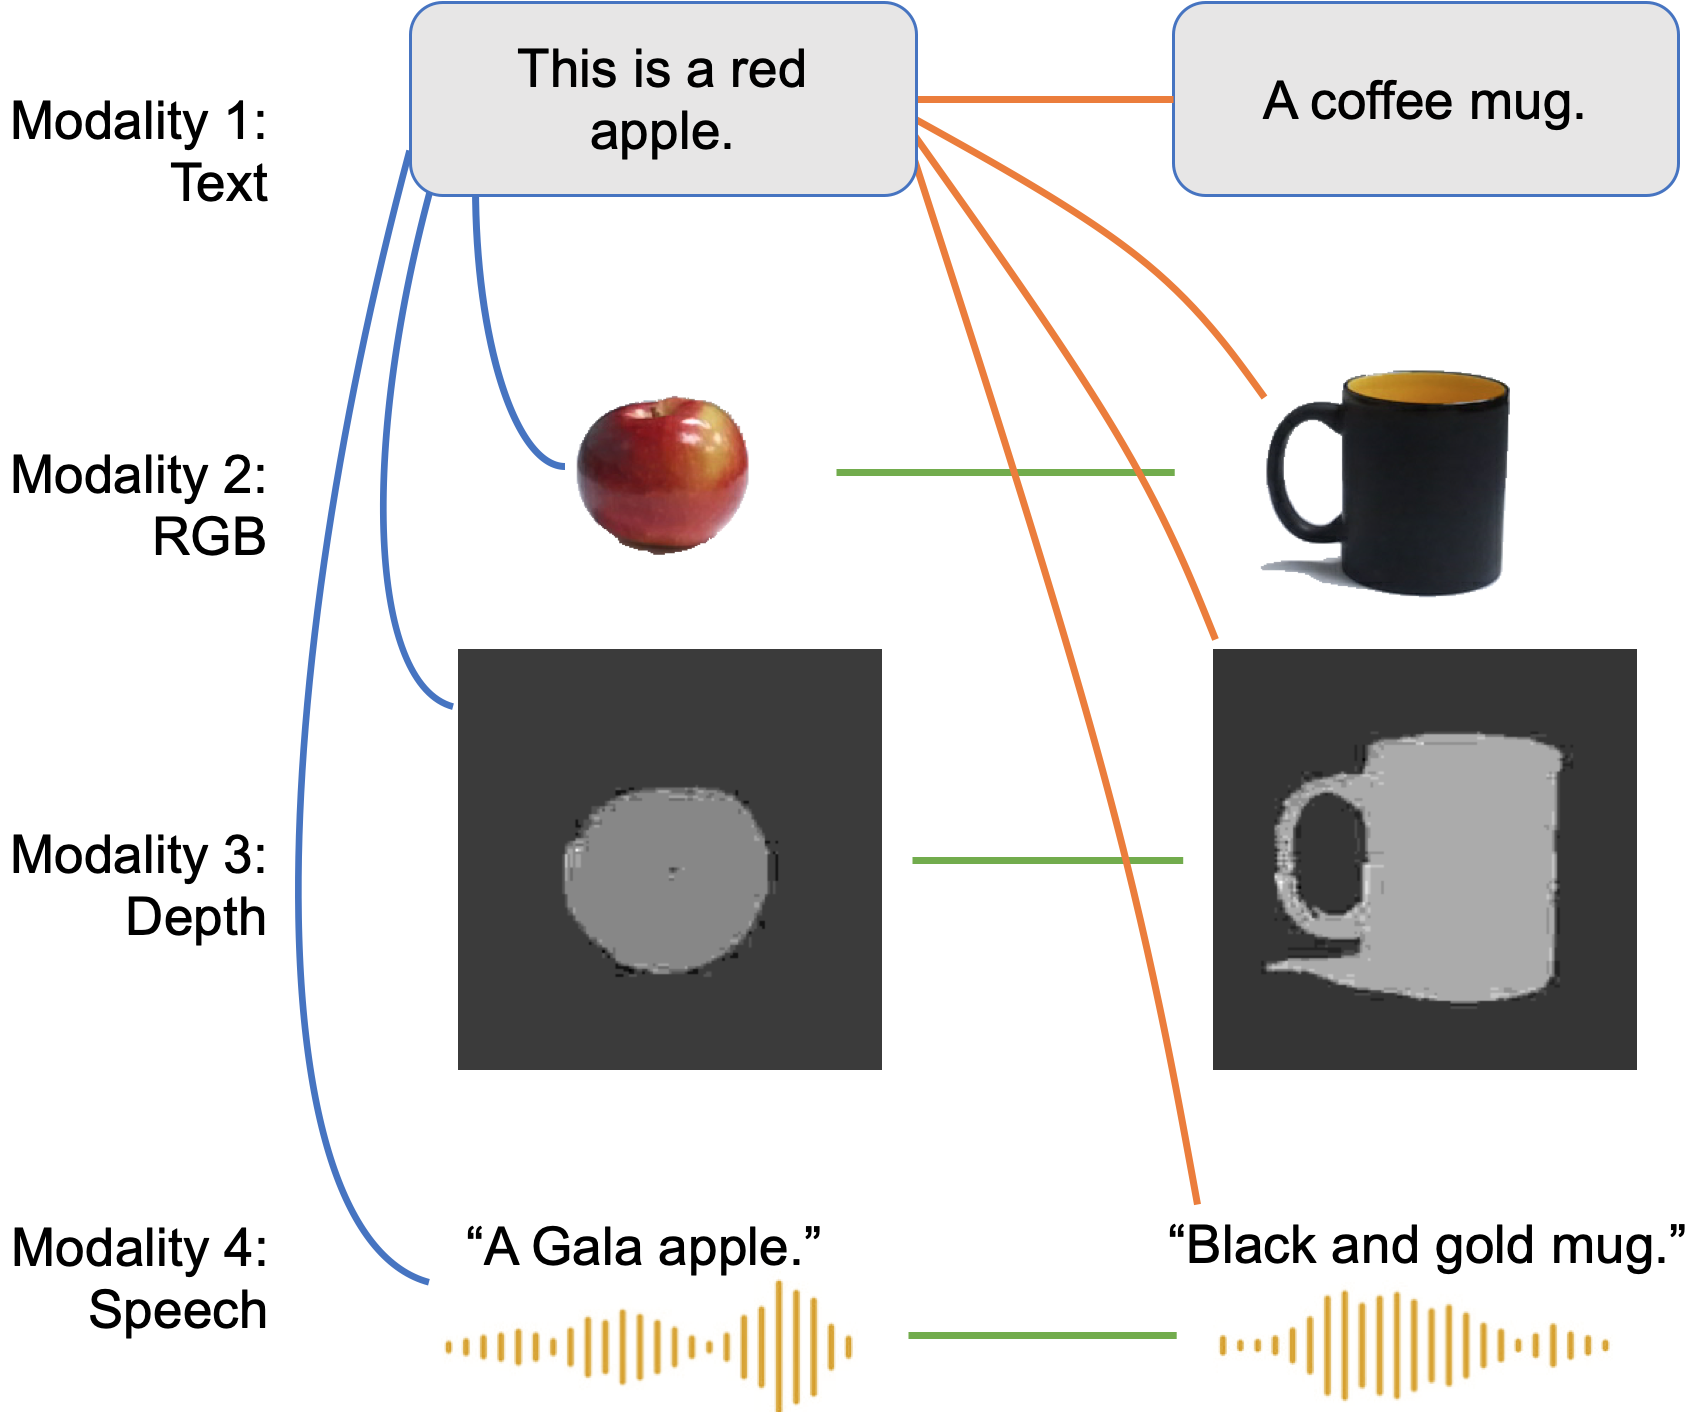
\includegraphics[width=.9\columnwidth]{Figures/4way-MMA.png}
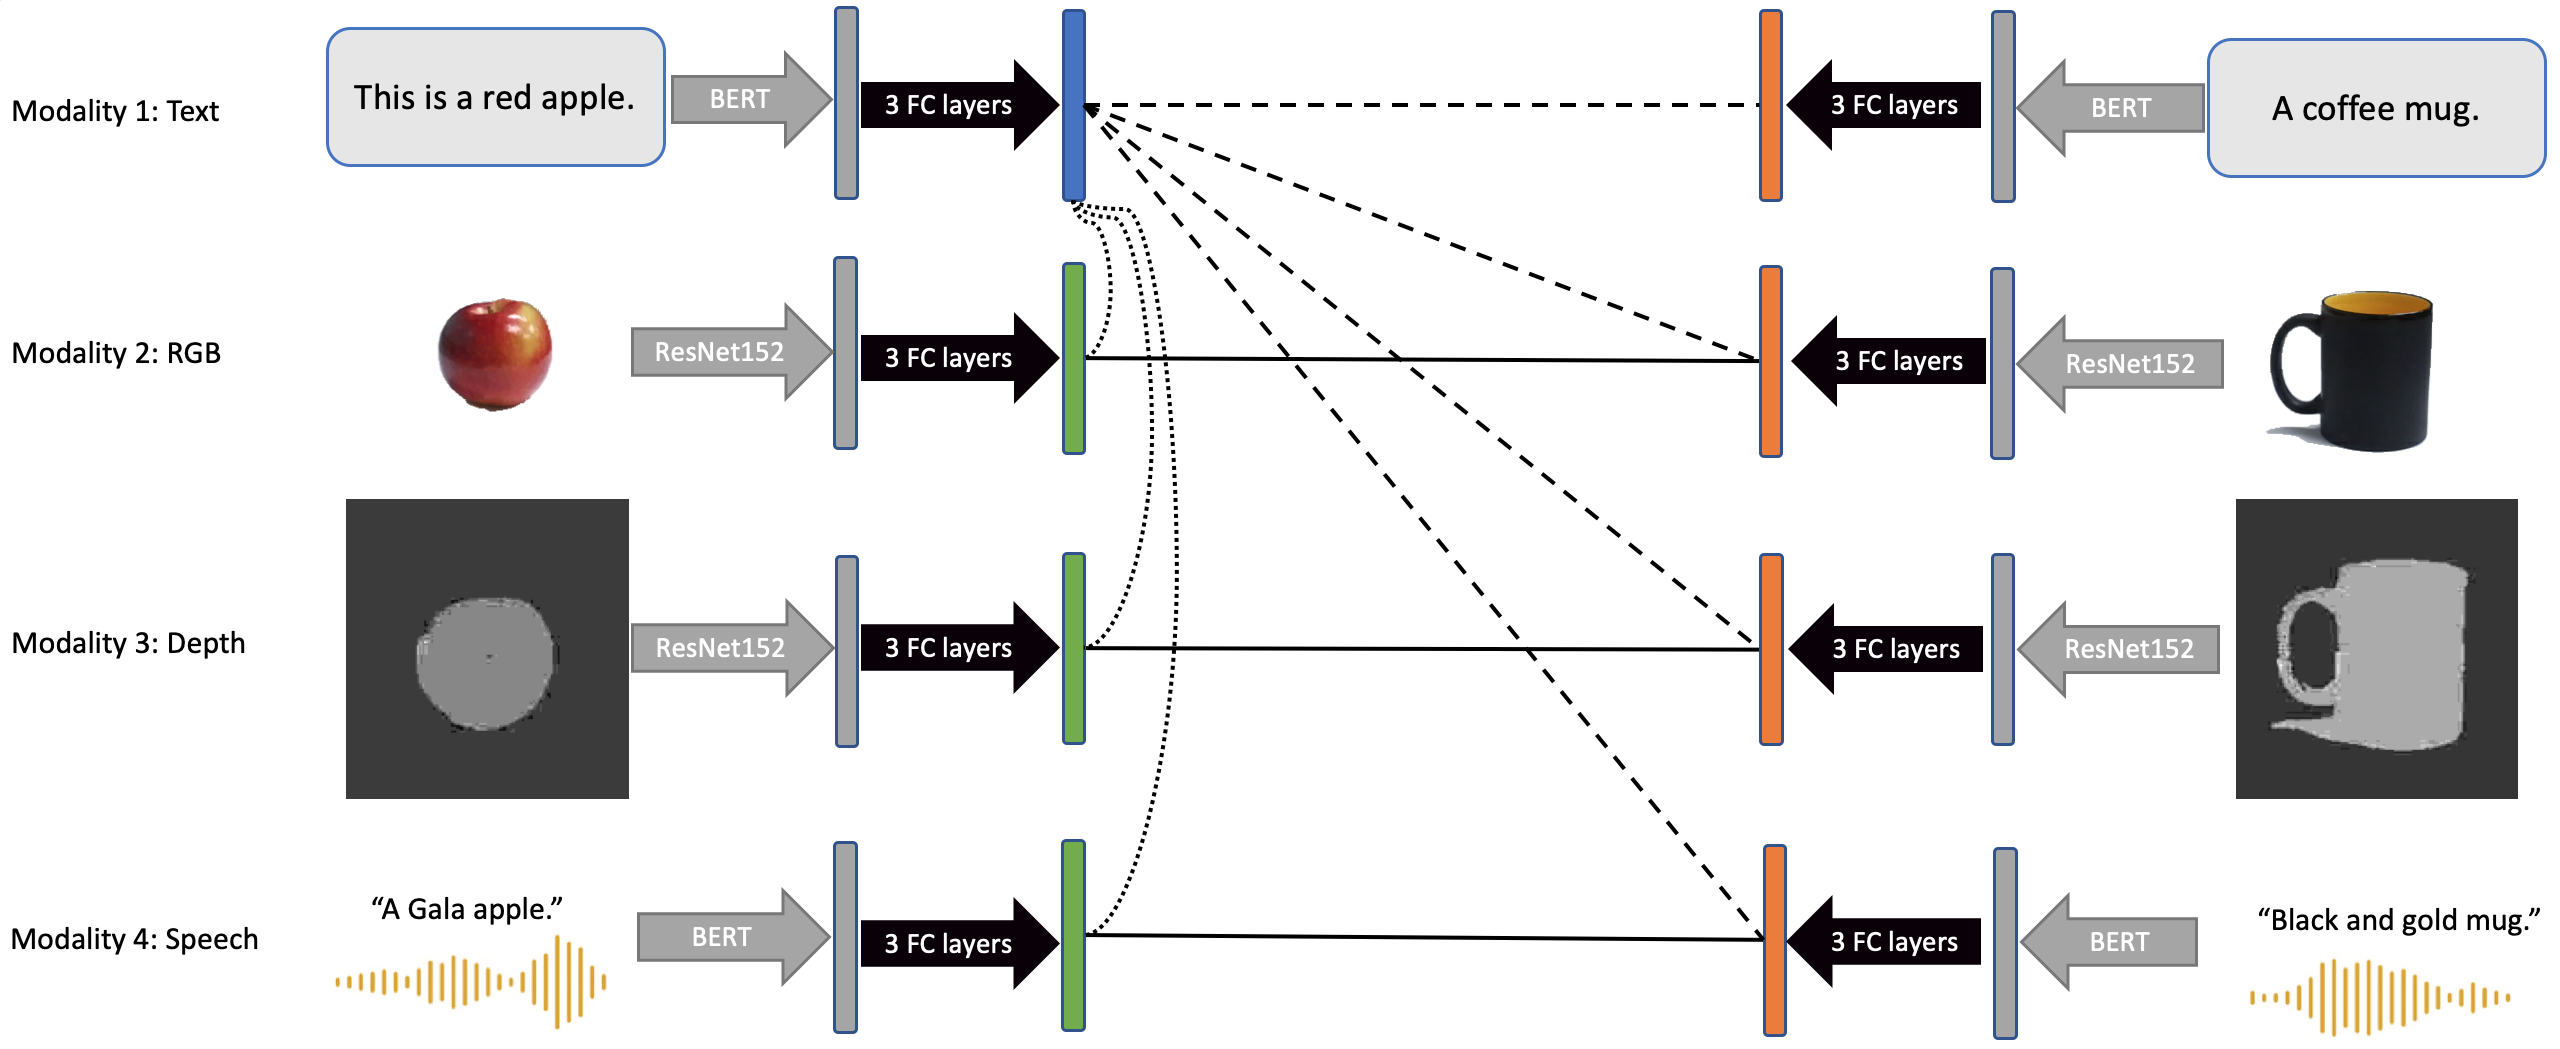
\includegraphics[width=2.1\columnwidth]{Figures/e-MMA.png}
\caption{A high-level prototype of our approach and the distances used in the MMA loss with four modalities. Gray arrows indicate pre-trained models that are frozen (i.e. the parameters are fixed and are not trained). The black arrows show 3 fully connected layers with a ReLU activitation function~\cite{relu2010} after the first two layers. These networks are trained.
Orange vectors are negative data points, green vectors are positive data points, and the blue vector is the anchor (which is the text modality of the positive data points).
Dashed lines indicate distances to be maximized, dotted lines indicate distances to be minimized, and solid lines show the enforced margin.
}
\label{fig:emma-loss}
\end{figure*}


\subsection{Network Architecture}
\label{sec:Model}

Transformers are de facto architectures in natural langauge processing community and have shown great success across different tasks. Similar to~\citet{GoLD_UMBC}, we use BERT~\cite{devlin-etal-2019-bert} embeddings contained in the FLAIR library ~\cite{akbik2019flair,akbik-etal-2019-pooled} to featurize the textual input, and wav2vec2~\cite{wav2vec2} to extract audio embeddings from speech. Both of these encoders output a 3072-dimensional embedding vector which is generated by concatenating the last four hidden layers of their corresponding networks. Both BERT~\cite{devlin-etal-2019-bert} and wav2vec2~\cite{wav2vec2} are self-supervised language models using transformers~\cite{vaswani2017attention}.
% \todo[inline]{A couple of sentences about FLAIR and wav2vec2 and what they do}

To process images, we use ResNet152~\cite{He_resnet_2016} for both RGB and depth images which gives us a 2048-dimensional embedding vector. Depth images are colorized before passing to the ResNet152.
We then use 3 fully connected layers with ReLU activation~\cite{relu2010} to map these embeddings to a shared 1024-dimensional space where we can compute the distances between all embeddings.




%===================================================================


\section{Experiments}
\label{sec:Experiments}

In this section we evaluate the quality of object retrieval models learned using the EMMA loss function. We first describe the dataset we use, give the metrics by which we evaluate the performance, the setup of the experiments, the baselines we compare against, and we end the section by a presenting results and analyzing them.

\subsection{Data}
\label{sec:Data}

We demonstrate the effectiveness of our approach on a recent multimodal dataset called GoLD~\cite{GoLD_UMBC}, which contains RGB image, depth image, written text descriptions, speech descriptions, and transcribed speech descriptions for 207 object instances across 47 object classes (see \cref{fig:emma-loss}). There are a total of 16,500 speech and 16,500 textual descriptions. The original GoLD paper uses raw RGB and raw depth images in which other objects are present in the background. We use a masked version of the images where the background is deleted (we observe that a masked version converges faster, however, they both converge to the same performance). Speech is converted to 16 Hz to match the wav2vec2 speech model~\cite{wav2vec2}.


\subsection{Problem Setup and Metrics}
\label{sec:metrics}
To evaluate our model we measure different performance metrics on a retrieval task where the model has to select an object among 5 objects given a language description. Only one of the objects corresponds to the description and the rest are from different object classes (e.g., one apple among a set including a fork, a mug, a lemon, and a bell pepper).


\subsubsection{Setup}
\label{sec:setup}
Similar to~\citet{NEURIPS2020_supervised_contrastive}, we use a stochastic gradient descent (SGD) optimizer with momentum~\cite{ruder2016overviewSGD} with a flexible learning rate starting at 0.05. 
For the triplet loss experiments we use the Adam~\cite{kingma_adam_2015} optimizer with scheduling learning rate as suggested by the papers.
The models are trained for 200 epochs with a batch size of 64 on a Quadro RTX 8000 GPU.


To evaluate the performance, we compute the distance between the given natural language description and 5 randomly selected images (1 of which corresponds to the description, with the others from different object classes). We compute the distance between one textual language embedding and all candidate RGB embeddings, and we compute the distance between the same language embedding and all candidate depth embeddings corresponding to the RGB embeddings. We then take average of these two distance matrices. Instead of choosing an empirical threshold beyond which objects are considered to be `referred to,' we choose the closest image embedding (average distance of RGB and depth from language) as the prediction.
In order to use cosine \textit{distance}, we have to subtract the cosine of the \textit{angle} between two embeddings (which represents similarity) from 1: that is, we compute $1 - \cos(e_1, e_2)$.

\subsubsection{Metrics}

The best metric to capture the performance in such a scenario is mean reciprocal rank (MRR, \cref{eq:mrr} for $Q$ queries). For each query we predict the rank of all objects based on their distance from the language command, and then the inverse rank of the desired objects in all queries are averaged. For example, if the model predicts the desired object as the first rank, then MRR = $\frac{1}{1} = 1$ which means a perfect score, and if it predicts the correct object as the last rank among five objects, then MRR = $\frac{1}{5}=0.2$. 

\begin{equation} \label{eq:mrr}
    \mathrm{MRR}=\frac{1}{|Q|} \sum_{i=1}^{|Q|} \frac{1}{\operatorname{rank}_{i}}
\end{equation}

Accuracy and micro F1 score
% (sklearn), flattened binary f1 score (sklearn), and F1 score 
are the same in this task, since for each prediction we either have a true positive and no false positives and no false negatives, or we have no true positives, one false positive and one false negative. MRR is a more informative metric because it captures the idea that having the correct object as the second choice should be considered better than having it as a last choice, while in accuracy the score is ``all or nothing''---either 0 or 1. Because our approach is designed to be robust to missing information across modalities, we also report MRR for different combinations of modality dropouts. 


\subsection{Baselines}
We compare our EMMA model against different contrastive learning methods including triplet loss, the traditional version of contrastive loss usually used in self-supervised settings~\cite{chen2020simple}, and supervised contrastive learning~\cite{NEURIPS2020_supervised_contrastive}. 



\begin{table*}[]
\centering
\begin{tabular}{lc|ll|lll}
\multicolumn{1}{c}{} &  & \multicolumn{2}{c|}{\textbf{Accuracy}} & \multicolumn{3}{c}{\textbf{Mean Reciprocal Rank}} \\ \hline
\multicolumn{1}{c|}{\textbf{Method}} & \textbf{Modalities} & \multicolumn{1}{c|}{\textbf{\begin{tabular}[c]{@{}c@{}}Speech/RGB/\\ Depth\end{tabular}}} & \multicolumn{1}{c|}{\textbf{\begin{tabular}[c]{@{}c@{}}Text/RGB/\\ Depth\end{tabular}}} & \multicolumn{1}{c|}{\textbf{\begin{tabular}[c]{@{}c@{}}Speech/RGB/\\ Depth\end{tabular}}} & \multicolumn{1}{c|}{\textbf{\begin{tabular}[c]{@{}c@{}}Text/RGB/\\ Depth\end{tabular}}} & \multicolumn{1}{c}{\textbf{\begin{tabular}[c]{@{}c@{}}Text/Speech/\\ RGB/Depth\end{tabular}}} \\ \hline
\multicolumn{1}{l|}{EMMA} & 4 & \multicolumn{1}{l|}{\textbf{0.65}$\pm$0.01} & 0.83$\pm$0.006 & \multicolumn{1}{l|}{\textbf{0.79}$\pm$0.002} & \multicolumn{1}{l|}{0.90$\pm$0.003} & 0.90$\pm$0.004 \\
\multicolumn{1}{l|}{EMMA} & 3 & \multicolumn{1}{l|}{--} & 0.84$\pm$0.008 & \multicolumn{1}{l|}{--} & \multicolumn{1}{l|}{0.90$\pm$0.004} & -- \\
\multicolumn{1}{l|}{Supervised Contrastive} & 4 & \multicolumn{1}{l|}{0.59$\pm$0.007} & 0.84$\pm$0.008 & \multicolumn{1}{l|}{0.75$\pm$0.004} & \multicolumn{1}{l|}{0.91$\pm$0.006} & 0.90$\pm$0.006 \\
\multicolumn{1}{l|}{Supervised Contrastive} & 3 & \multicolumn{1}{l|}{--} & 0.84$\pm$0.006 & \multicolumn{1}{l|}{--} & \multicolumn{1}{l|}{0.91$\pm$0.004} & -- \\
\multicolumn{1}{l|}{Contrastive Cosine} & 4 & \multicolumn{1}{l|}{0.40$\pm$0.153} & 0.83$\pm$0.006 & \multicolumn{1}{l|}{0.62$\pm$0.034} & \multicolumn{1}{l|}{0.90$\pm$0.004} & 0.89$\pm$0.005 \\
\multicolumn{1}{l|}{Contrastive Cosine} & 3 & \multicolumn{1}{l|}{--} & 0.84$\pm$0.005 & \multicolumn{1}{l|}{--} & \multicolumn{1}{l|}{0.91$\pm$0.003} & -- \\
\multicolumn{1}{l|}{Triplet} & 3 & \multicolumn{1}{l|}{--} & 0.83$\pm$0.008 & \multicolumn{1}{l|}{--} & \multicolumn{1}{l|}{0.90$\pm$0.005} & -- \\ \hline
\end{tabular}
\caption{Average and standard deviation of accuracy and MRR over 3 runs with 3 different random seeds on a held-out test set. These results represent performance when no modalities are ablated, in which case supervised contrastive loss, contrastive loss, and EMMA perform similarly (``--'' is an ablated modality and can't be evaluated). All metrics are from 0 to 1, and higher is better. For 5 objects, a random guess would have MRR of 0.33, and the worst case performance would be always ranking the correct item last which gives us 0.2. All models are trained using text as anchor. The batch size is 64 and optimizer is SGD for all experiments except the triplet loss, where batch size is 1 and optimizer is Adam.}
\label{table:quantitative}
\end{table*}
% %Edward moved table above where refernced b/c LaTeX plays games with double-wide objects
% \begin{table*}[bth]
% \centering
% \begin{tabular}{c|c|c|c|c|c|c}
% \toprule
% \textbf{Method} & \textbf{Modalities} & \textbf{acc.srd} & \textbf{acc.trd} & \textbf{MRR.srd} & \textbf{MRR.trd} & \textbf{MRR.tsrd} \\ %\hline
% \midrule
% EMMA (Text) & 4 & \textbf{0.65}$\pm$0.01 & 0.83$\pm$0.006 & \textbf{0.79}$\pm$0.002 & 0.90$\pm$0.003 & 0.90$\pm$0.004 \\
% EMMA (Text) & 3 & - & 0.84$\pm$0.008 & - & 0.90$\pm$0.004 & - \\
% % Simple MMA (Text)  & 3 & ?$\pm$? & ?$\pm$? & ? & ? \\
% % Simple MMA (Text) & 4 & ?$\pm$? & ?$\pm$? & ? & ? \\
% % Simple MMA (Speech) & 3 & ?$\pm$? & ?$\pm$? & ? & ?  \\
% DONE Supervised Contrastive (Text)& 4 & 0.59$\pm$0.007 & 0.84$\pm$0.008 & 0.75$\pm$0.004 & 0.91$\pm$0.006 & 0.90$\pm$0.006  \\
% TODO Supervised Contrastive (Text)& 3 & - & 0.84$\pm$0.006 & - & 0.91$\pm$0.004 & -\\
% DONE Contrastive Cosine (Text) & 4 & 0.40$\pm$0.153 & 0.83$\pm$0.006 & 0.62$\pm$0.034  & 0.90$\pm$0.004 & 0.89$\pm$0.005\\
% TODO Contrastive Cosine (Text) & 3 & - & 0.84$\pm$0.005 & -  & 0.91$\pm$0.003 & -\\
% PROJ Triplet (Text) & 3 & - & 0.83$\pm$0.008 & - & 0.90$\pm$0.005 & -  \\
% % DONE EMMA (Speech) & 3 & ?$\pm$? & ?$\pm$? & - & - \\
% % DONE EMMA (Speech) & 4 & ?$\pm$? & ?$\pm$? & ? & ? \\
% % DONE Supervised Contrastive (Speech)& 3 & ?$\pm$? & ?$\pm$? & - & -\\
% % DONE Supervised Contrastive (Speech)& 4 & ?$\pm$? & ?$\pm$? & ? & ? \\
% % TODO Contrastive Cosine (Speech) & 3 & ?$\pm$? & ?$\pm$?  & - & -\\
% % TODO Contrastive Cosine (Speech) & 4 & ?$\pm$? & ?$\pm$?  & ? & ?\\
% % DONE Triplet (Speech) & 3 & ?$\pm$? & ?$\pm$? & - & -  \\

% % Full MMA (Text) w/ neg & 3 & ?$\pm$? & ?$\pm$? \\
% % Simple MMA (Text) w/ neg Adam & 3  & 0.7949$\pm$? & 0.8778$\pm$? \\
% % Simple MMA (Text) w/ neg SGD & 3 & 0.7905$\pm$? & 0.8821$\pm$? \\
% % Triplet (Text) w/ neg & 3 & 0.7497$\pm$? & 0.8522$\pm$? \\
% % Full MMA (Speech) w/ neg & 3 & ?$\pm$? & ?$\pm$? \\
% % Simple MMA (Speech) w/ neg & 3 & 0.7949$\pm$? & 0.8778$\pm$? \\
% % Contrastive Cosine (Text) w/ neg & 3 & 0.7894$\pm$? & 0.8788$\pm$?  & ? & ?\\
% % Contrastive (Speech) w/ neg & 3 & ?$\pm$? & ?$\pm$? \\
% % Triplet (Speech) w/ neg & 3 & 0.7497$\pm$? & 0.8522$\pm$? \\
% \bottomrule
% \end{tabular}
% \caption{\label{table:quantitative}Average and standard deviation of accuracy and MRR over 3 runs with 3 different random seeds on a held-out test set. These results represent performance when no modalities are ablated, in which case supervised contrastive loss, contrastive loss, and EMMA perform similarly. All metrics are from 0 to 1, and higher is better. For 5 objects, a random guess would have MRR of 0.33, and the worst case performance would be always ranking the correct item last which gives us 0.2. All models are trained using text as anchor. The batch size is 64 and optimizer is SGD for all experiments except the triplet loss, where batch size is 1 and optimizer is Adam.
% % \todokdinline{maybe adding results on cropped and raw dataset as well. Also results using object class instead of negative sampling}
% }
% \end{table*}

\subsubsection{Triplet Loss}
\label{sub:baseline-triplet}
The triplet loss function consists of three data points including anchor, positive, and negative from two modalities. The anchor, positive, and negative can be chosen from different modalities in each batch.
The triplet loss method has two major disadvantages. First, it cannot be used for more than two modalities. Second, a batch size of greater than 1 is hard to implement if the anchor, positive, and negative come from different modalities for each batch.
% To address these issues in EMMA, we sample more than one positive and negative data points.
To address these issues in EMMA, we choose one modality as anchor. Intuitively, we sample one positive data point and one negative data point from each modality, resulting in 2M data points. The anchor data point is always from the same modality and corresponds to the same object class sampled for positive data points. \Cref{table:quantitative} shows that our MMA method perform as good as this baseline while out model can be trained 10x faster since we can use batch sizes larger than 1. Also, our method can be used for any number of modalities, while previous works~\cite{GoLD_UMBC,triplet_loss_2021_CVPR} concatenate rgb and depth to form a single vector to handle more than two modalites.
When we used a fixed anchor modality, a batch size of 64, and applied semantic negative sampling~\cite{Pillai_Matuszek_2018}, our method outperformed this baseline. However, since this method cannot be applied to four modalities, we do not include it in the main analysis.
Moreover, our method has the advantage that does not require triplet mining or providing hard examples.

\subsubsection{Contrastive Loss}
\label{sub:baseline-contrastive}

We compare our model against contrastive loss. In order to implement this loss function, we use cosine similarity as suggested in the SimCLR paper~\cite{chen2020simple}. Another possibility is to use an inner dot product~\cite{NEURIPS2020_supervised_contrastive}; this can lead to instabilities since the dot product is not bounded. This contrastive loss function is formulated in \cref{eq:contrastive-loss}:
% \todokdinline{try contrastive loss with cross-entropy, dot product, and the supervised contrastive method itself (without triplets).}

% Original Formula
\begin{equation}\label{eq:contrastive-loss}
    -\sum_{i \in I} \log \frac{\exp (sim(z_i , z_{j(i)}) / \tau) }{\sum_{a \in A(i)} \exp (sim(z_i, z_a) / \tau)}
\end{equation}
% \begin{equation}\label{eq:contrastive-loss}
%     -\sum_{i \in I} \log \frac{\exp (sim(f(x_i) , z_{j(i)}) / \tau) }{\sum_{a \in A(i)} \exp (sim(f(x_i), f(x_a)) / \tau)}
% \end{equation}
where $i$ is anchor, $j(i)$ is the set of positives excluding anchor, $a$ is the set of all positives and negatives excluding anchor, and $z = f(x)$.

\Cref{eq:contrastive-loss} can be extended to the loss function formulated in \cref{eq:mma-contrastive}. Our formulation is a generalized version of the contrastive loss where $M$ is the number of modalities (e.g. RGB image, depth image, speech, text), but it can be ``augmented views'' instead of different modalities.

\begin{equation}\label{eq:mma-contrastive}
    -\sum_{m=1}^{M-1} \log \frac{\exp (sim(z_a^+ , z_{m}^{+})/ \tau) }{ \exp (sim(z_a^+ , z_{m}^{+}) / \tau) + \exp (sim(z_a^+, z_{m}^{-}) / \tau)}
\end{equation}
where $z = f(x)$.


\subsubsection{Supervised Contrastive Learning}
\label{sub:baseline-supcon}

\citet{NEURIPS2020_supervised_contrastive} propose a supervised way of performing contrastive learning which is shown in \cref{eq:supervised-contrastive}.

\begin{equation}\label{eq:supervised-contrastive}
    \sum_{i \in I} \frac{-1}{|P(i)|} \sum_{p \in P(i)} \log \frac{\exp (z_i \cdot z_p / \tau) }{\sum_{a \in A(i)} \exp (z_i \cdot z_a / \tau)}
\end{equation}

% \begin{equation}\label{eq:supervised-contrastive-my-notation}
%     \sum_{i \in I} \frac{-1}{|P(i)|} \sum_{p \in P(i)} \log \frac{\exp (f_i(x_i) \cdot f_p(x_p) / \tau) }{\sum_{a \in A(i)} \exp (f_i(x_i) \cdot f_a(x_a) / \tau)}
% \end{equation}




While this model is a strong baseline, if modalities are ablated, this method does not perform as well as our proposed model (we show and discuss this later, in \cref{fig:epochs-mrr.srd}). This is especially true when the text modality is dropped, as is likely in physical agent scenarios, where speech is a natural interaction mechanism.


\subsection{Modality Ablation}
We consider an experiment in which we incorporate RGB, depth, speech, and written language to train the model. The loss function requires no changes beyond increasing the value of $M$ by 1 in \cref{eq:objective-emma}. Our goal is the non-trivial downstream prediction task: determining what objects are being referred to by arbitrary language from a small number of examples. When we consider only text, RGB, and depth, written language is used as the anchor modality, and we compute the distance of RGB and depth modalities from it and then average them. However, when speech is incorporated as an additional fourth sensory modality, we have three possible choices. \textit{First}, we can compute the distance of RGB and depth from text and from speech which gives us 4 distance matrices, and then take average of these four. \textit{Second}, we can treat speech in a similar way to RGB and depth: compute the distance of RGB, depth, and speech from text, and then take an average of three of them. \textit{Third}, similar to the first method, but adding the distance between language and speech as well and then take the average of 5 distance matrices.

Of these, the first method is the most appropriate choice for a robust multimodal alignment approach. The second and third options are possible during training, but in real-world object retrieval scenarios, having only one form of language instructions is a reasonable scenario---people are not likely to \textit{both} speak about \textit{and} type in instructions for an agent. At test time, depending on which modalities are available to the model, we can use speech, text, or both to compute the distance of RGB and depth embeddings from the linguistic query, and then take the average.
\Cref{eq:distance-matrix} shows all possible cases of modality dropout and the corresponding distance computations, where ``t'' represents \textit{text}, ``s'' represents \textit{speech}, ``r'' represents \textit{RGB}, ``d'' represents \textit{depth}, $K_{ij}$ for each pair of modalities is the distance of one instance in modality $i$ from all instances in modality $j$, and $K$ is the final distance---a matrix if there are multiple queries and a vector if there is one query.
\begin{equation}
\label{eq:distance-matrix}
K = 
    \begin{cases} 
        K_{tr} & \text{speech and depth are missing} \\
        K_{sr} & \text{text and depth are missing} \\
        K_{td} & \text{speech and RGB are missing} \\
        K_{sd} & \text{text and RGB are missing} \\
        K_{trd} = \frac{K_{tr} + K_{td} }{2} & \text{speech is missing} \\
        K_{srd} = \frac{K_{sr} + K_{sd} }{2} & \text{text is missing} \\
        K_{tsr} = \frac{K_{tr} + K_{sr} }{2} & \text{depth is missing} \\
        K_{tsd} = \frac{K_{td} + K_{sd} }{2} & \text{RGB is missing} \\
        K_{tsrd} = \frac{K_{tr} + K_{td} + K_{sr} + K_{sd} }{4} & \text{o.w.} \\
    \end{cases}
\end{equation}


\Cref{fig:epochs-mrr.srd,fig:epochs-mrr.trd,fig:epochs-mrr.sd,fig:epochs-mrr.sr} show the relative performance of EMMA against baselines when different modalities are ablated.


\subsection{Results}
\label{sec:results}
In this section we provide quantitative and qualitative results by comparing our method against supervised contrastive learning~\cite{NEURIPS2020_supervised_contrastive} and na\"ive contrastive loss~\cite{chen2020simple}.
% We evaluate our EMMA loss function against the na\"ive triplet loss method. Our model significantly outperforms the triplet method across all epochs while it converges faster as shown in \cref{fig:epochs-mrr.srd}.
\Cref{table:quantitative} summarizes the performance of all models with different ablation metrics.
% \todo[inline]{Why do we call out triplet loss specifically? We evaluate against several baselines? I don't understand this section particularly}
To provide a better sense of the performance measure, we can think of a model that always ranks the correct object in the second place which is not very bad. Such a model would have MRR of $1/2 = 0.5$.


Comparing \cref{fig:epochs-mrr.trd} and \cref{fig:epochs-mrr.srd}, we can see that when the text modality is dropped the performance decreases from about 0.90 to about 0.79, showing that speech cannot completely replace the text. 
We also observe that speech has a higher variance compared to text, and a na\"ive contrastive learning method cannot take advantage of text modality to reduce this variance. While the other two methods leverage text modality to align speech better.

There is very little gap in performance when rgb is dropped in \cref{fig:epochs-mrr.sd} compared to when depth is dropped in \cref{fig:epochs-mrr.sr} which shows that our model is robust enough when rgb or depth sensors fail in real-world deployment.


\begin{figure}[tbh]
\centering
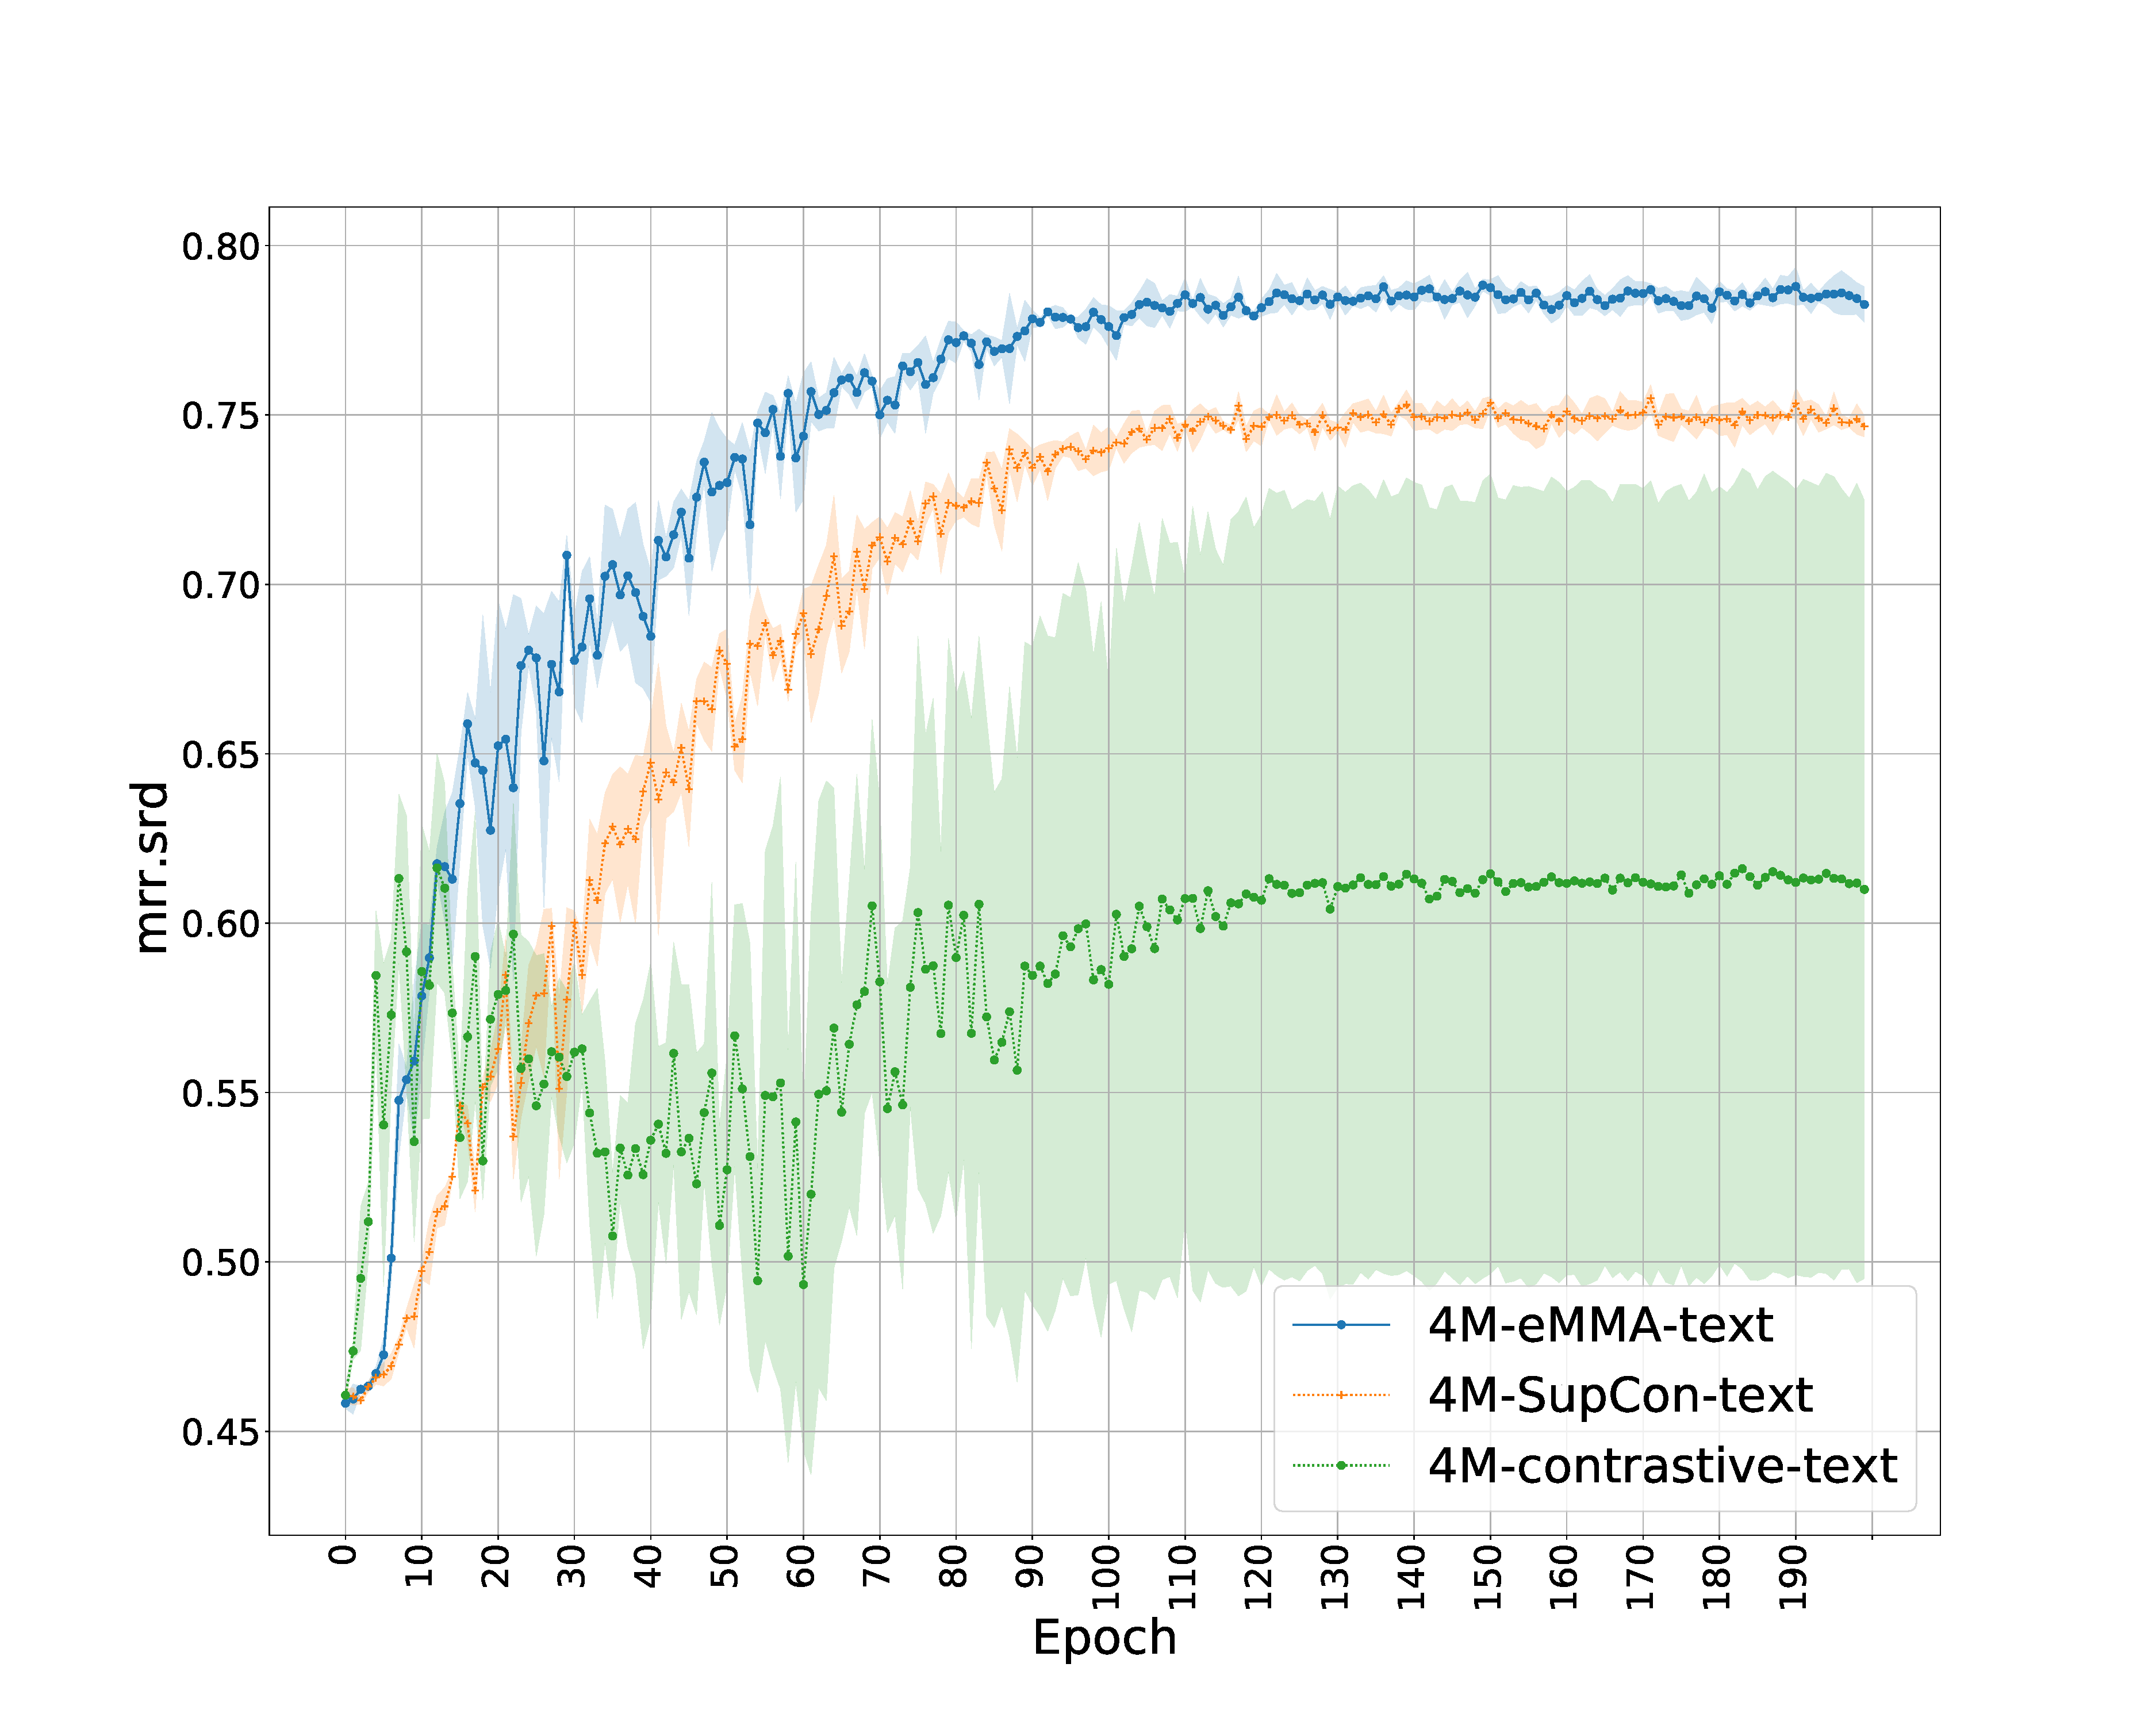
\includegraphics[width=.99\columnwidth]{Figures/average-seeds-epochs-mrr_ard.pdf}
\caption{Mean Reciprocal Rank (MRR) on the held-out test set when the text modality is ablated, averaged over 3 runs. Green is self-supervised contrastive learning, orange is supervised contrastive learning, and blue represents our proposed EMMA loss function. Higher is better.
% \todo[inline]{Fix description of colors.}
}
\label{fig:epochs-mrr.srd}
\end{figure}

\begin{figure}[tbh]
\centering
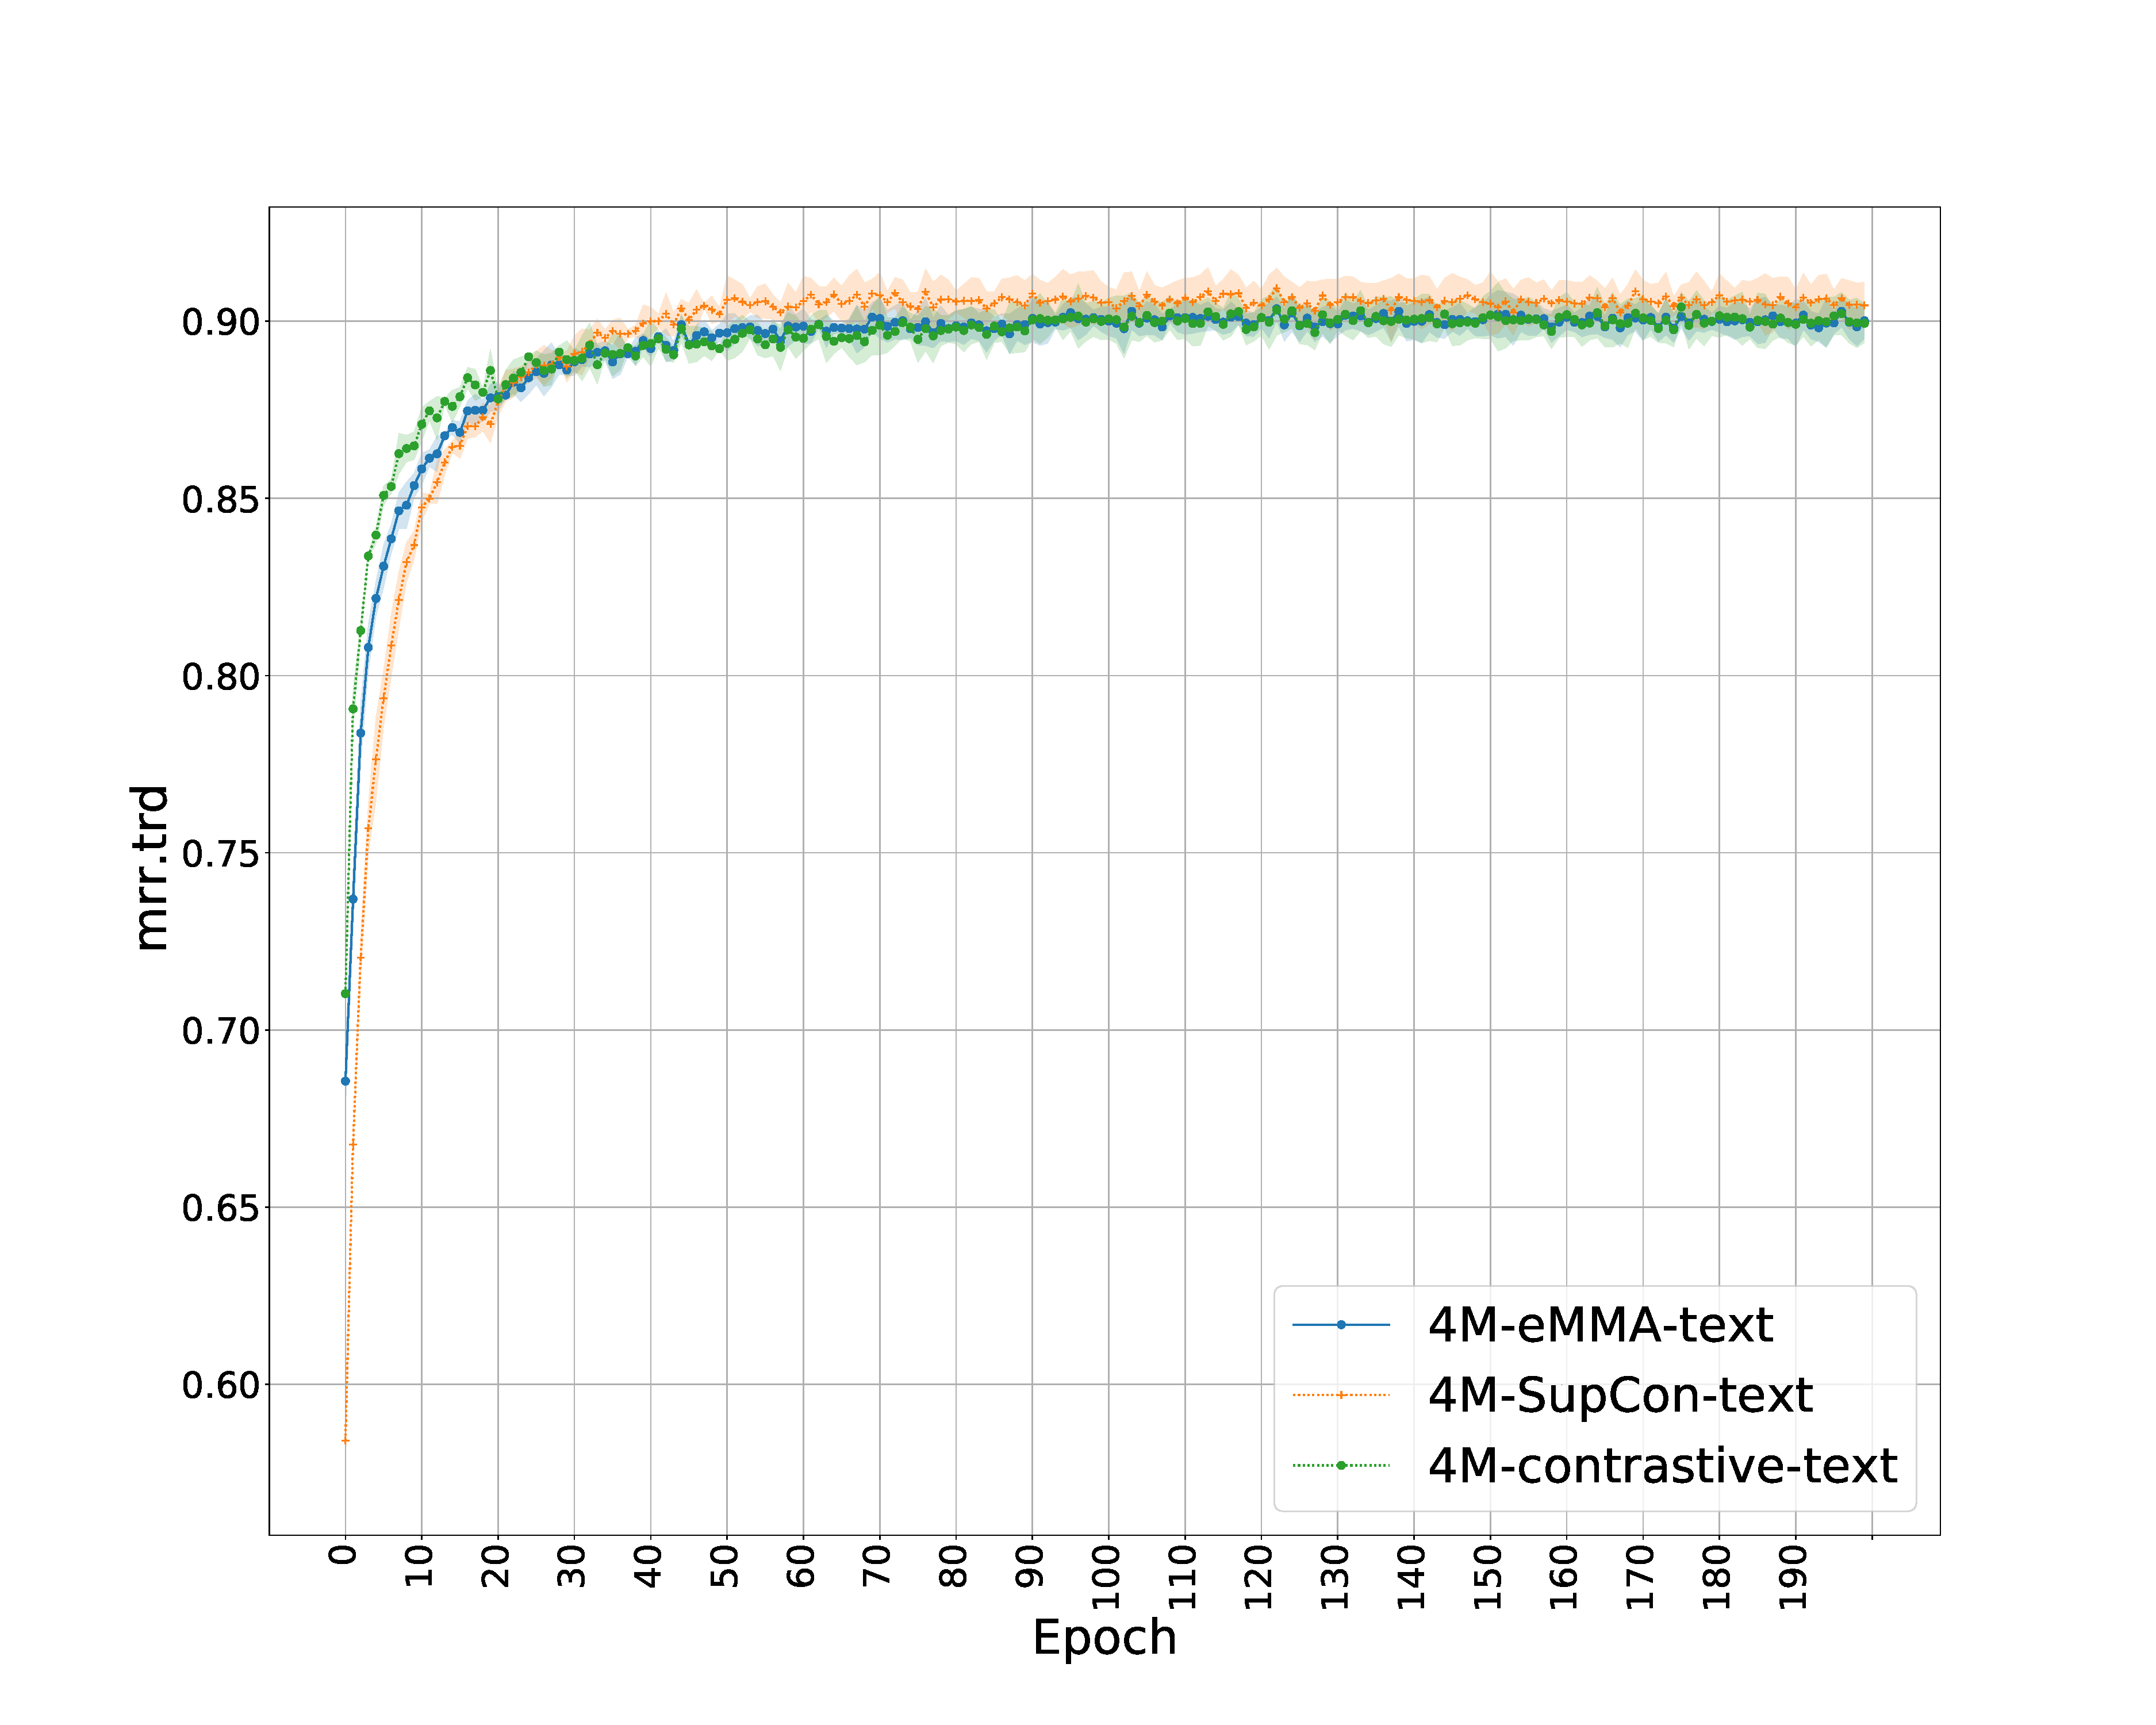
\includegraphics[width=.99\columnwidth]{Figures/average-seeds-epochs-mrr_lrd.pdf}
\caption{Mean Reciprocal Rank (MRR) on the held-out test set when the speech modality is ablated, averaged over 3 runs, for the downstream task of object retrieval. Green is self-supervised contrastive learning, orange is supervised contrastive learning, and blue represents our proposed EMMA loss function. Higher is better. When speech as a modality is ablated, all tested methods perform similarly.
}
\label{fig:epochs-mrr.trd}
\end{figure}


\begin{figure}[tbh]
\centering
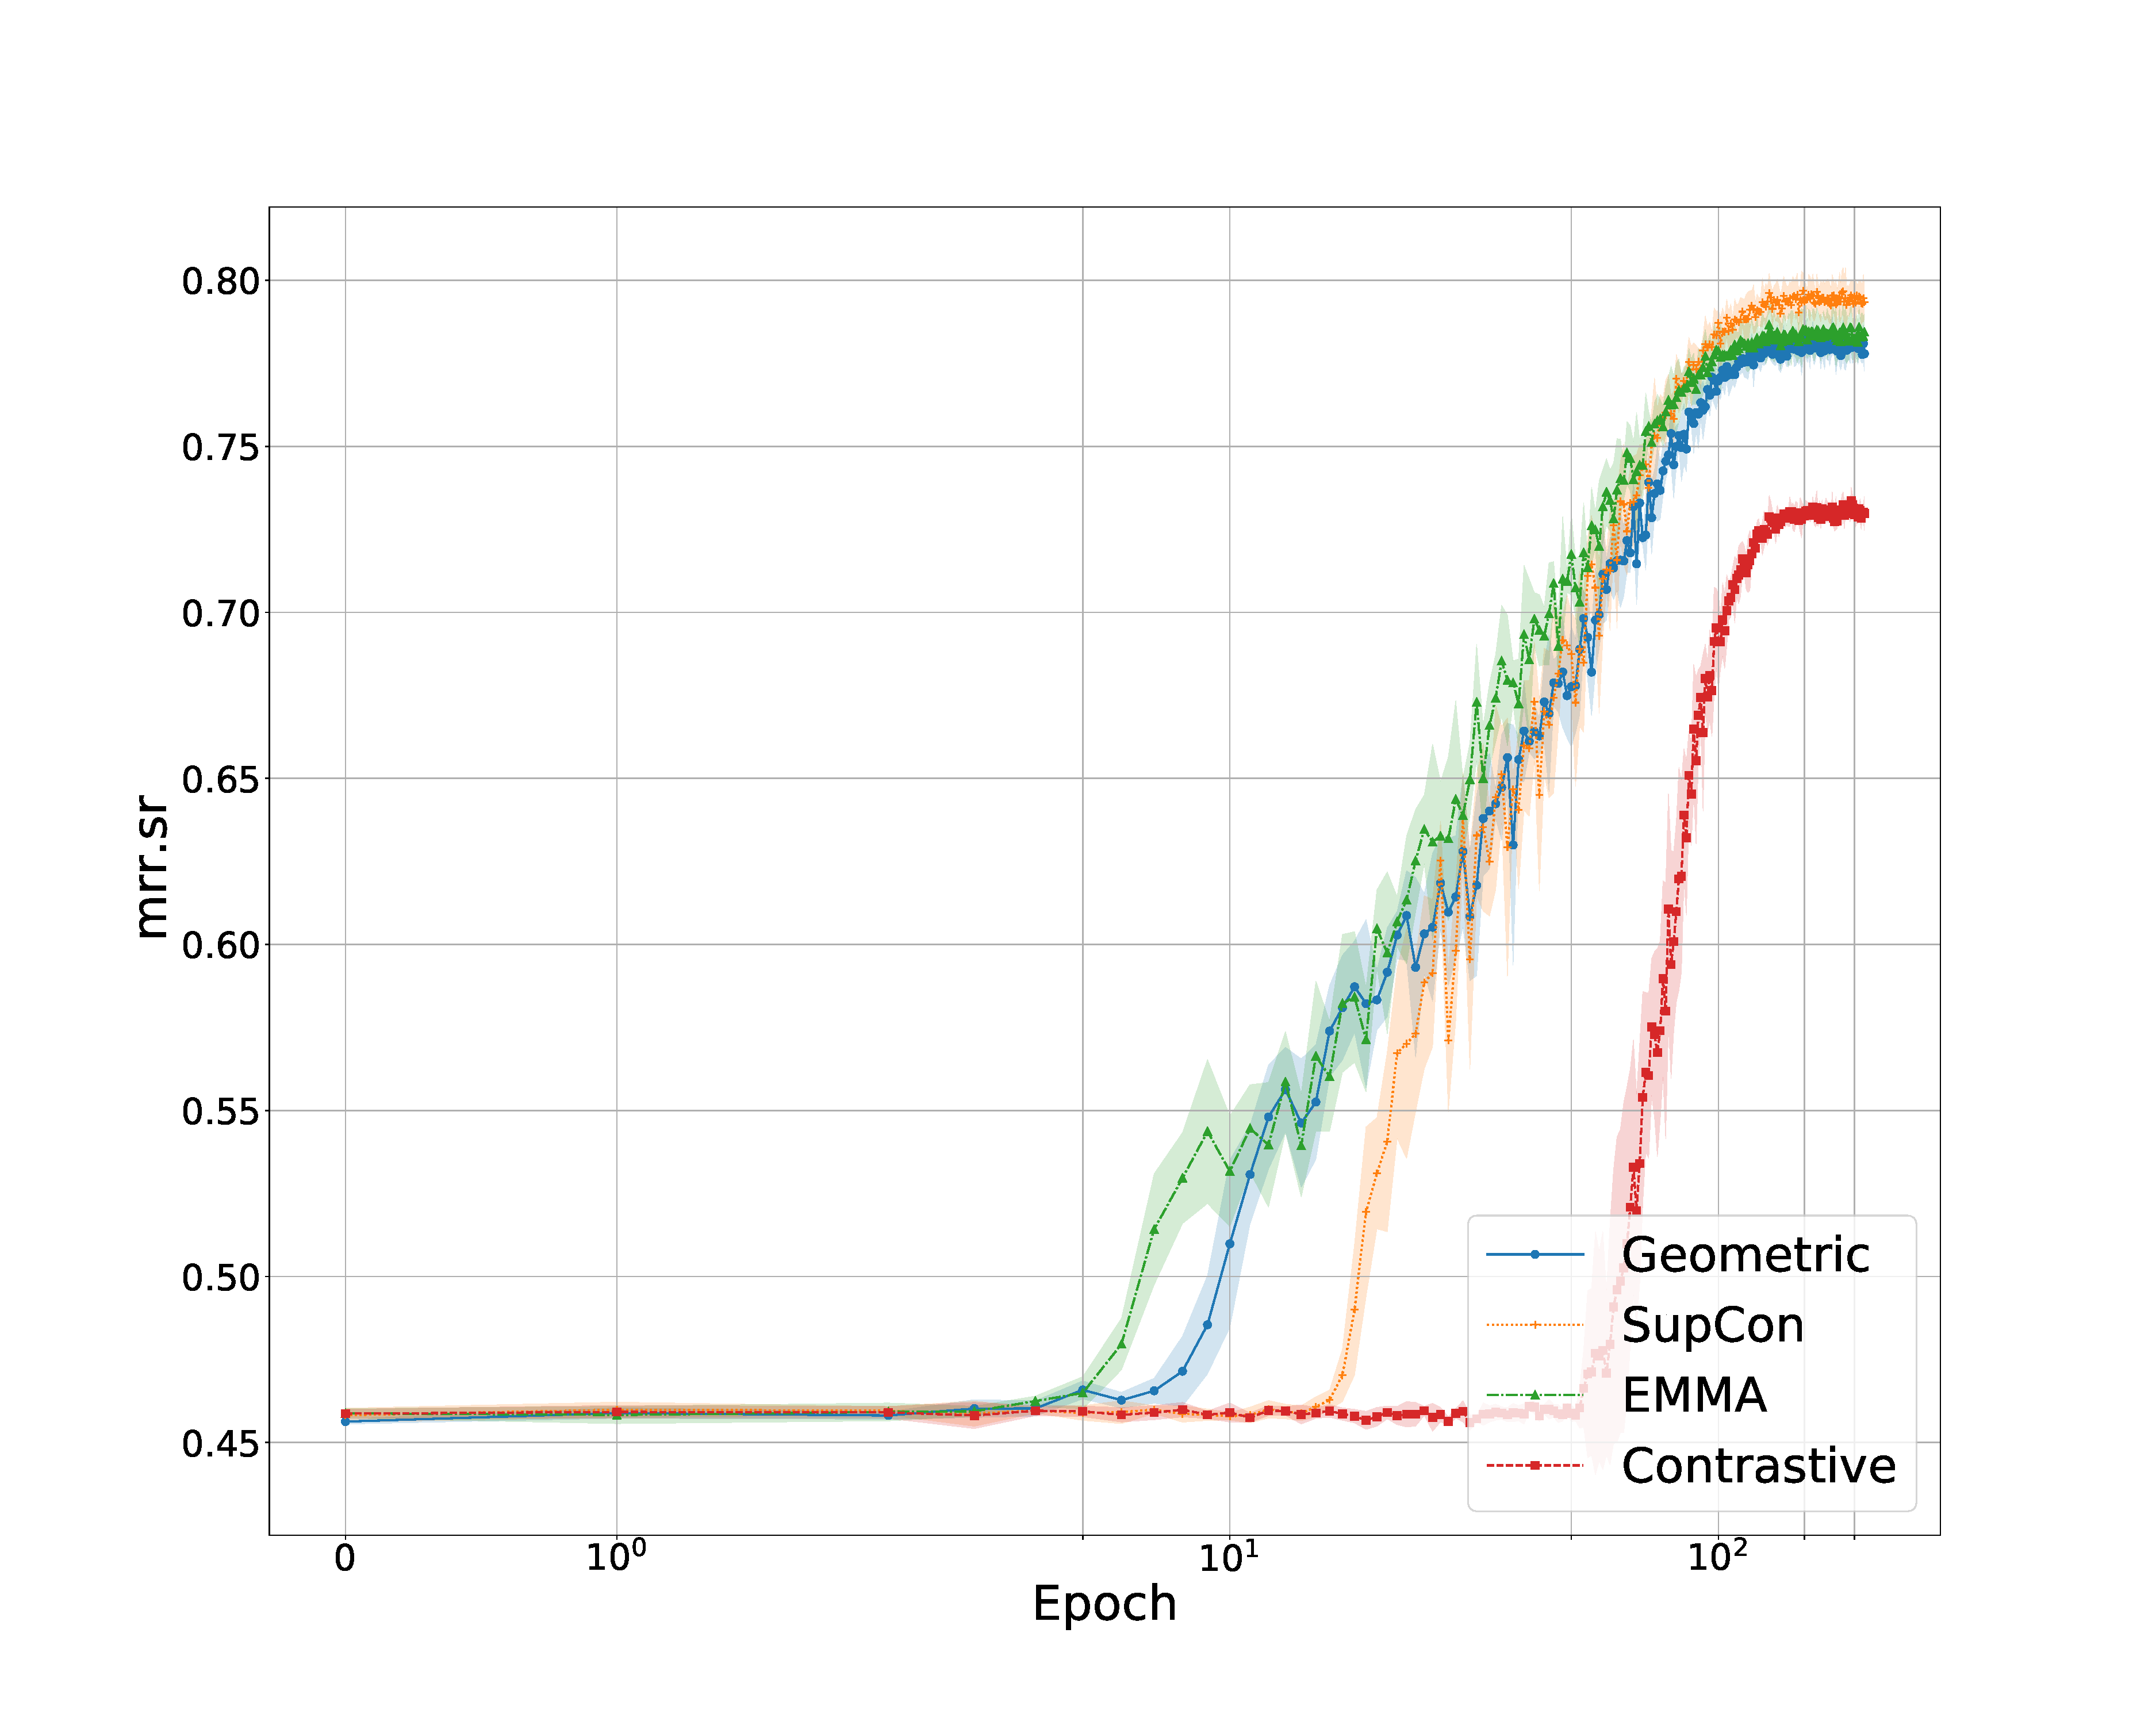
\includegraphics[width=.99\columnwidth]{Figures/average-seeds-epochs-mrr_ar.pdf}
\caption{Mean Reciprocal Rank (MRR) on the held-out test set when text and depth modalities are ablated, averaged over 3 runs for the downstream task of object retrieval.  Green is self-supervised contrastive learning, orange is supervised contrastive learning, and blue represents our proposed EMMA loss function. Higher is better.
% Orange represents Supervised Contrastive Learning~\cite{NEURIPS2020_supervised_contrastive}, \Complete{} represents the triplet loss function~\cite{triplet_loss_2021_CVPR}.
}
% \todocmi{Maybe MRR is wrong and we should be looking at top-ranked result?}
\label{fig:epochs-mrr.sr}
\end{figure}



\begin{figure}[tbh]
\centering
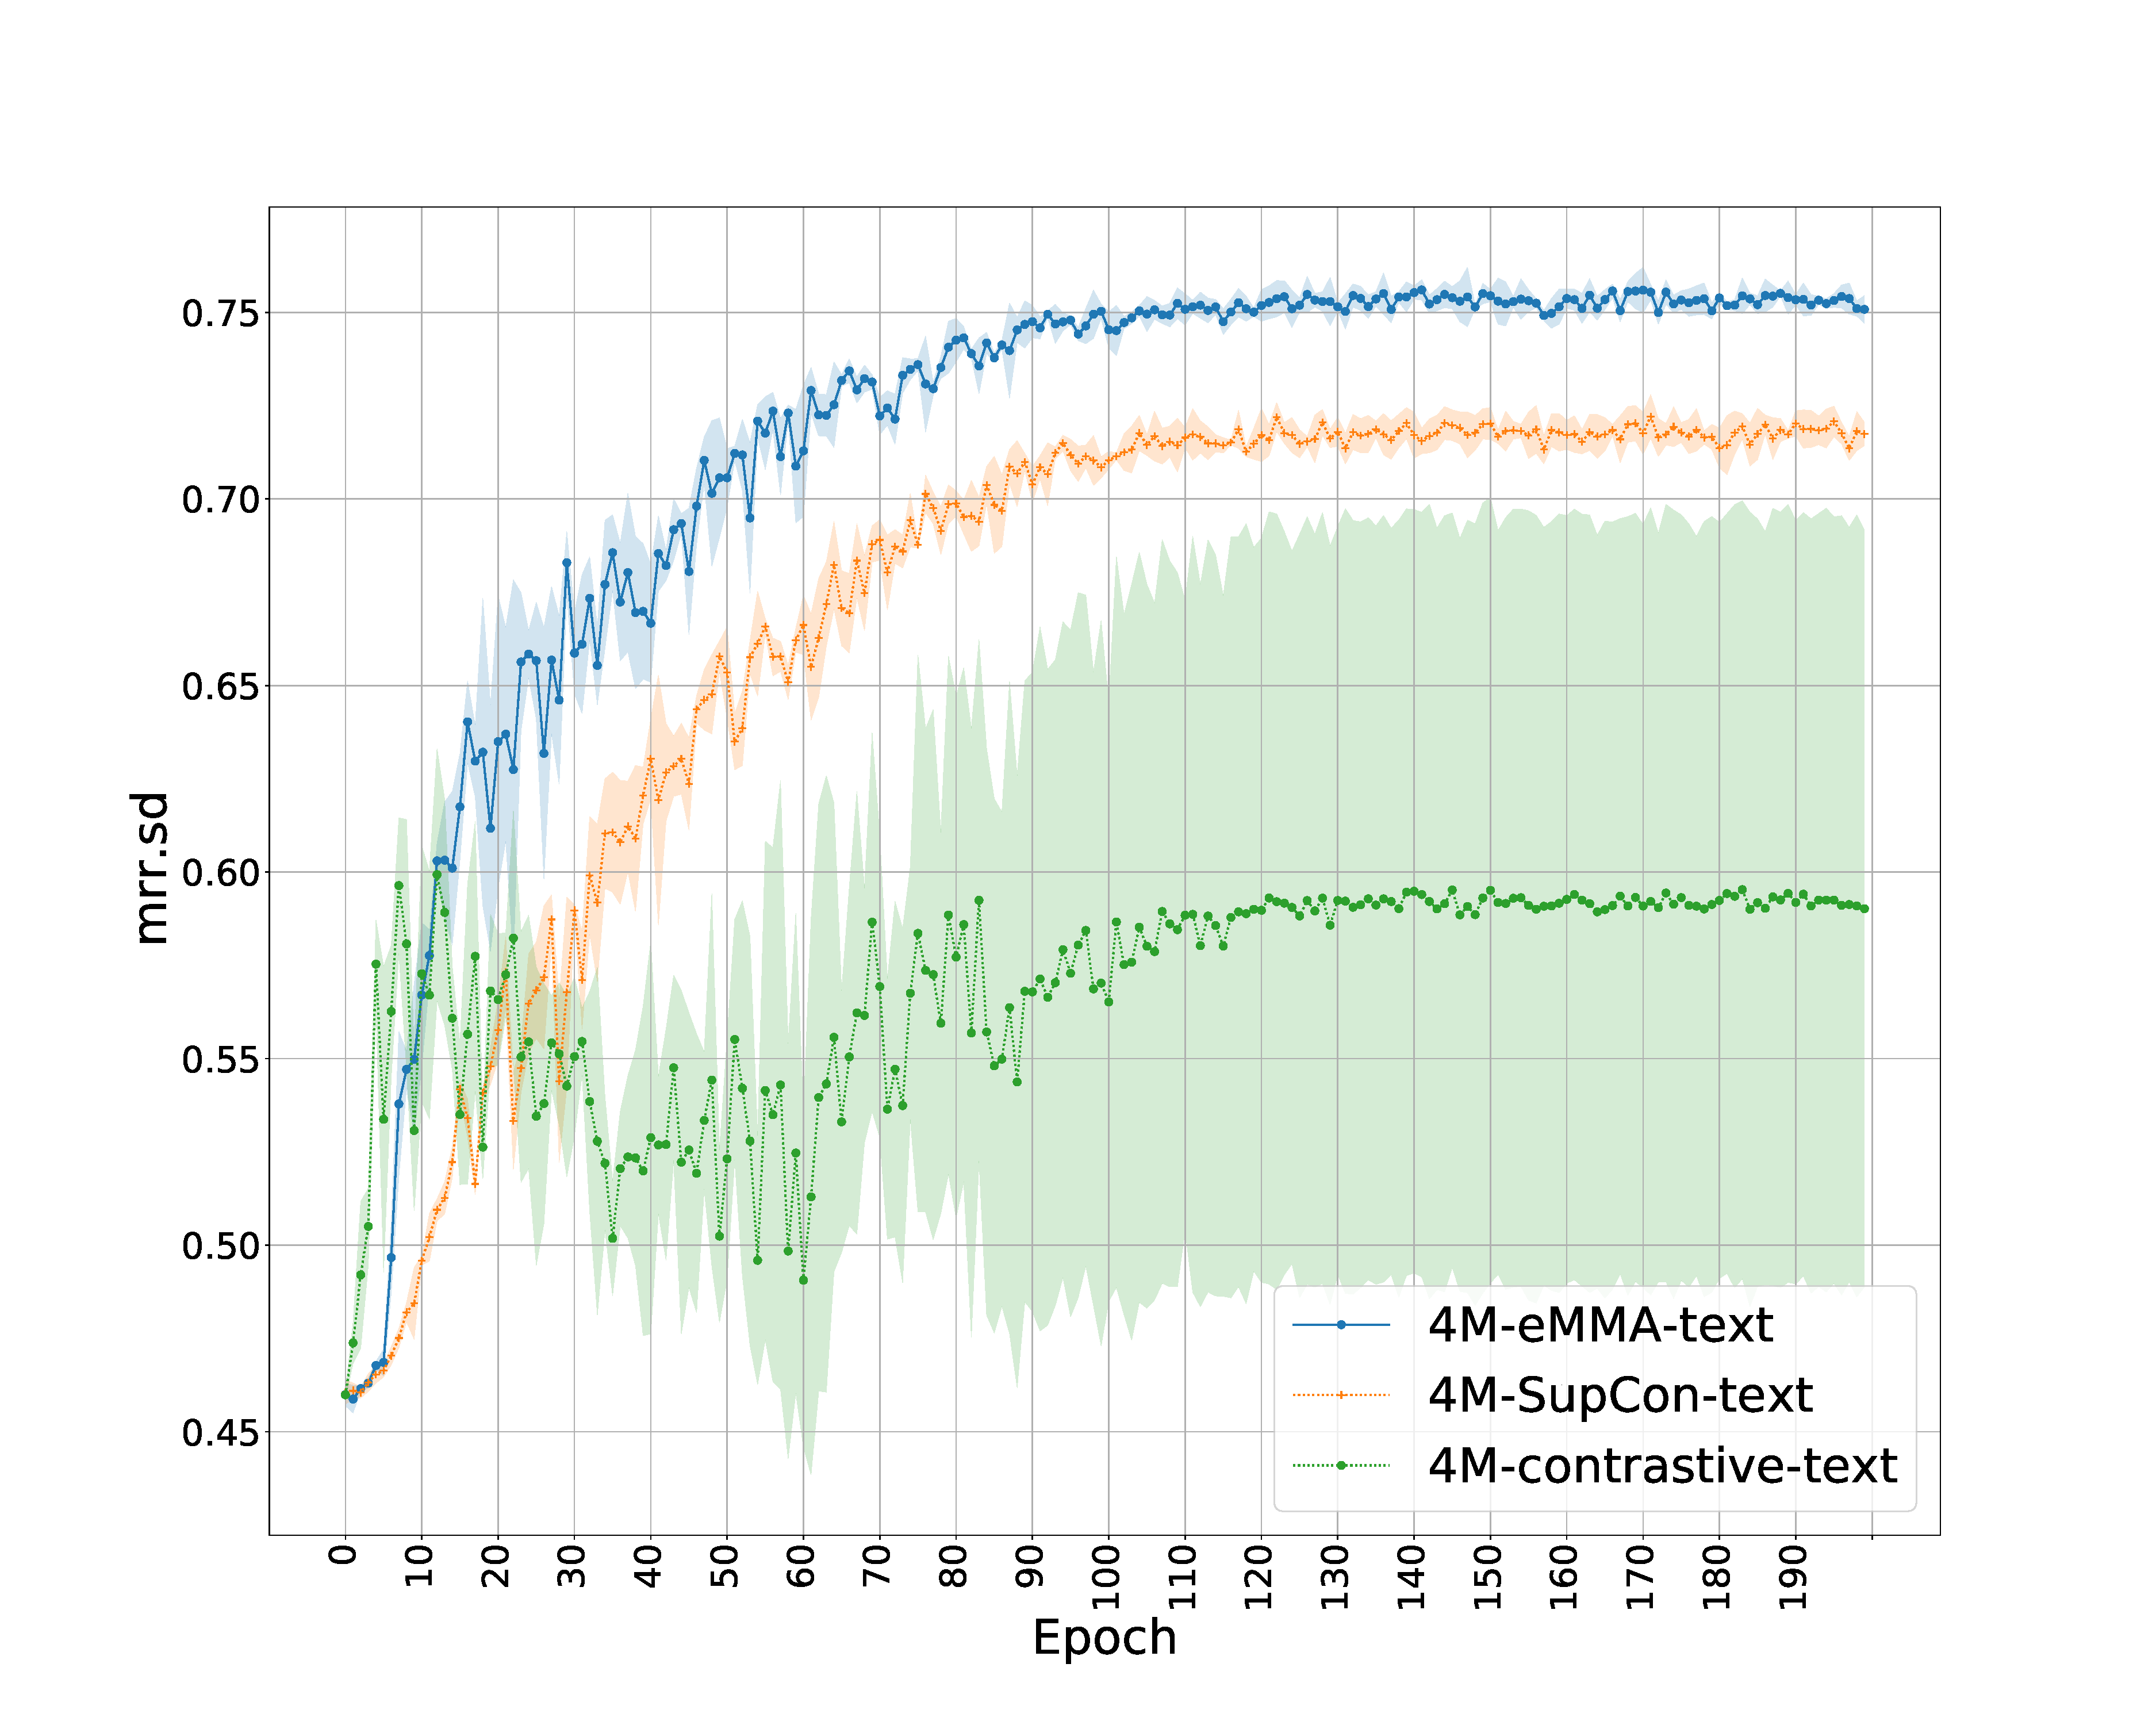
\includegraphics[width=.99\columnwidth]{Figures/average-seeds-epochs-mrr_ad.pdf}
\caption{Mean Reciprocal Rank (MRR) on the held-out test set when text and RGB modalities are dropped averaged over 3 runs for the downstream task of object retrieval.  Green is self-supervised contrastive learning, orange is supervised contrastive learning, and blue represents our proposed EMMA loss function. Higher is better.
}
\label{fig:epochs-mrr.sd}
\end{figure}

\begin{figure*}[tbh]
\centering
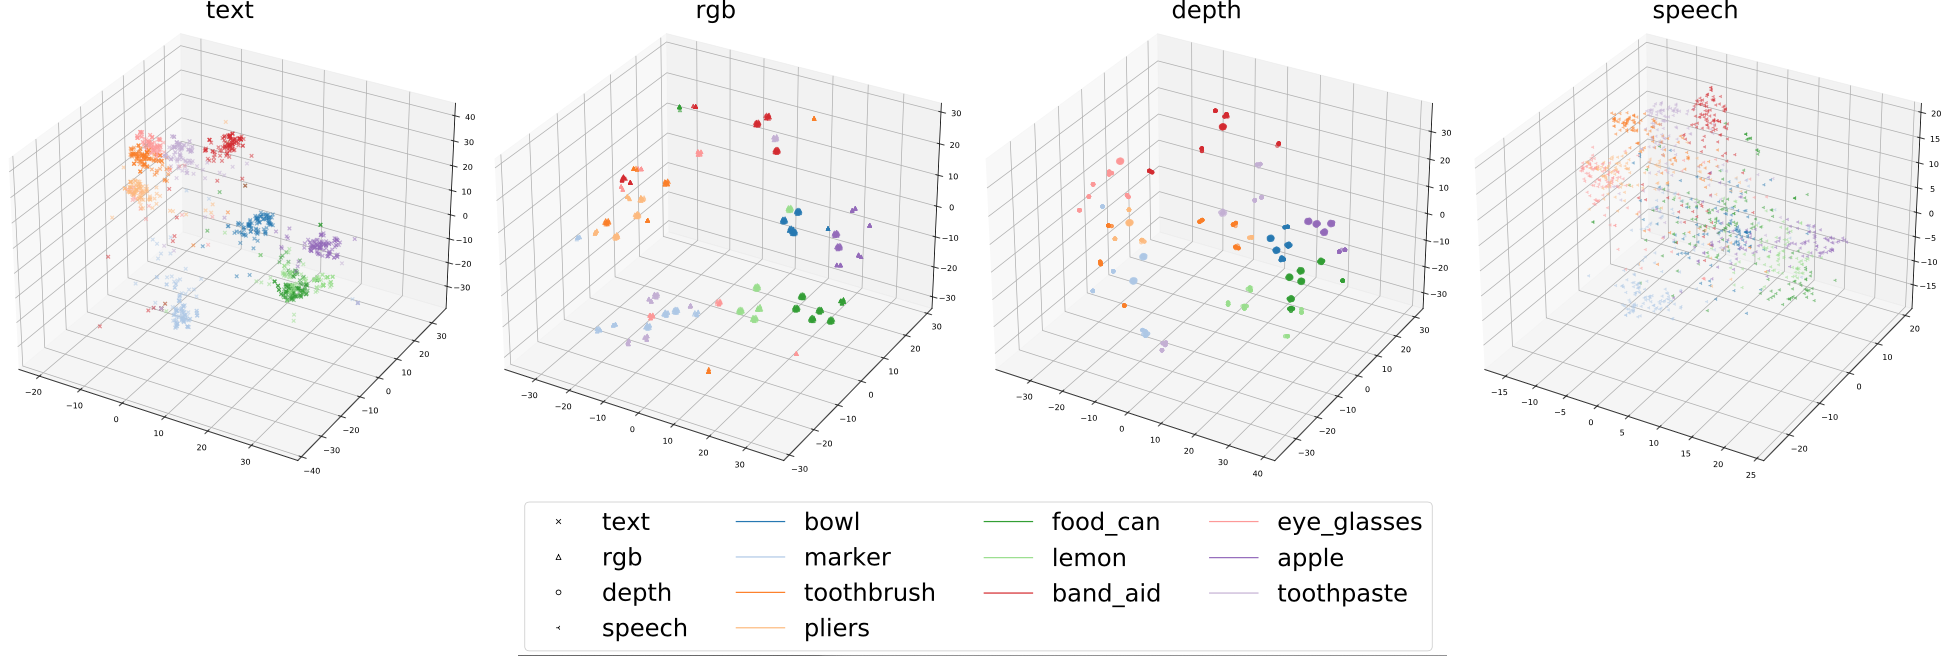
\includegraphics[width=1.99\columnwidth]{Figures/3D-tsne-4M-eMMA-cosine-submodalities-text-anchor-gold-no_neg_sampling-1024-sbs.png}
\caption{3D T-SNE~\cite{van2008tsne} projection of test embeddings of 10 randomly selected classes of objects using our proposed method EMMA. Each modality is separately projected into a three-dimensional space. In a perfect embedding, all instances of a class would be clustered in identical areas of the embedding space across all modalities. We can see that EMMA successfully encourages all four modalities to live in a common manifold, allowing accurate retrieval even when modalities are missing. 
}
\label{fig:3d-tsne}
\end{figure*}

% \subsection{Qualitative Results}
% \label{sec:Qualitative}
We look into the projection of the high-dimensional learned embeddings into a 2-dimensional and 3-dimensional spaces using t-SNE~\cite{van2008tsne}, which is a dimensionality reduction technique to visualize high-dimensional data. T-SNE creates a probability distribution over pairs high-dimensional data where similar pairs have a higher probability and dissimilar pairs have a lower probability. A similar probability distribution is also defined over pairs of data in the lower dimension (either 2D or 3D), and T-SNE minimizes the KL divergence between these two probability distributions.
% \textcolor{red}{\dots}\todo{explanation}. 
% \Cref{fig:2d-tsne} shows the projection of all test embeddings from all different modalities in a 2D space. As shown in the graph, instances of the same class but different modality are mapped to almost the same locations and are closer to each other.
\Cref{fig:3d-tsne} shows the projection onto 3D space to give a better view of the location of embeddings. Although these projections are not perfect, combined with the quantitative results, they demonstrate that our model is learning to map instances of the same class closer to each other regardless of their modalities.


% \begin{figure}[tbh]
% \centering
% 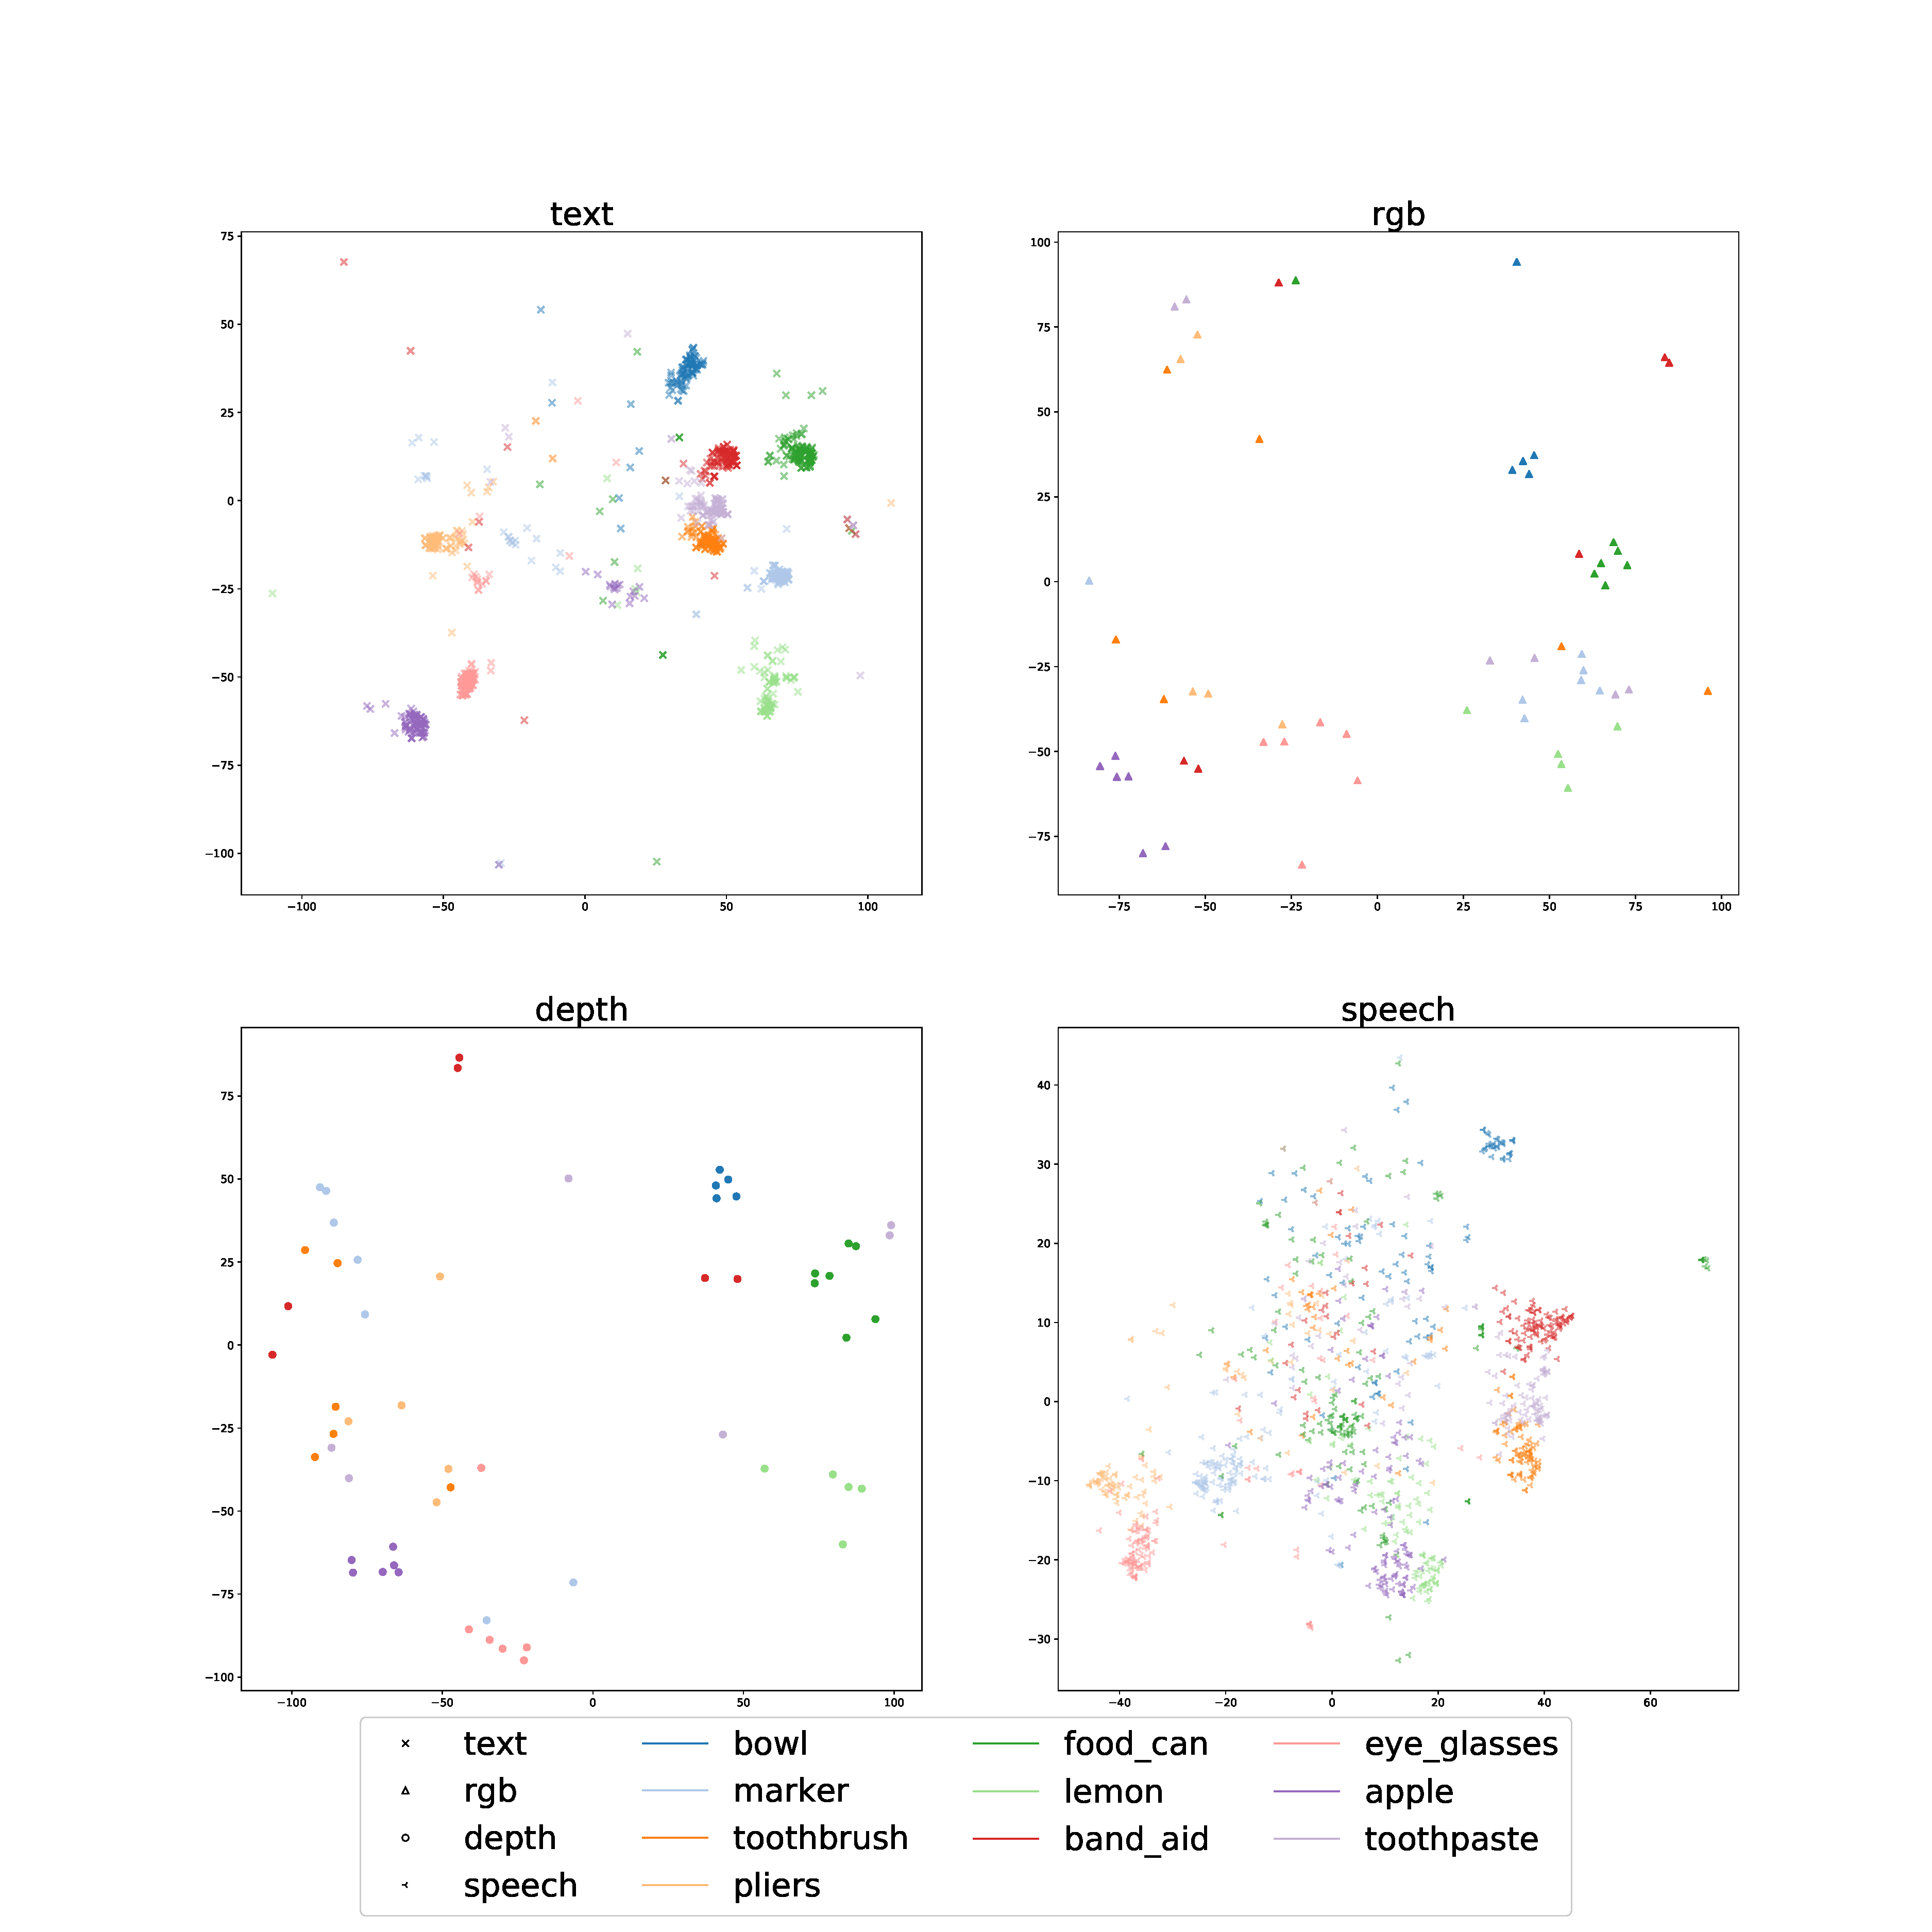
\includegraphics[width=.99\columnwidth]{Figures/2D-tsne-4M-eMMA-cosine-submodalities-text-anchor-gold-no_neg_sampling-1024.pdf}
% \caption{2D T-SNE~\cite{van2008tsne} projection of test embeddings of 10 randomly selected classes of objects using our proposed method. Each modality is separately projected into a two-dimensional space. \Rephrase{} \textcolor{red}{We may only want 3D}
% }
% \label{fig:2d-tsne}
% \end{figure}

% \todokdinline{Add the T-SNE projection for supervised contrastive loss as well.}

% \subsection{Failed Experiments}
% \todokdinline{I suppose I should remove this subsection, right?}
% We tried a lot of different approaches and they did not work better than our model or the baselines, but we list them here to save time for readers who want to try them.

% \subsubsection{Simple MMA}
% Copy text from \ref{sub:simple-mma} if we decide to keep this section.

% \subsubsection{Two Anchors}
% Since speech is similar to text in its usage when it comes to the downstream task of object retrieval (given a single language command, find the correct object among multiple objects), we decided to have text and speech as two anchors instead of having one anchor only. When there is one anchor, the distance between positive pairs text and speech is minimized and the distance between negative pairs are minimized. However, this is not related to the downstream task since we never want to find the correct speech for a given text or vice versa. The second term added to the last function is exactly similar to the loss function when speech is the anchor, and the first term is the same as when language is the anchor. Therefore, the performance is somewhere in the middle of those two approaches but more towards the speech when the metrics are computed based and speech matrices.

% \subsection{Example Prediction}



\subsection{Discussion}
Our proposed model performs well, has been demonstrated to handle four modalities of shared information effectively, and is robust to test-time situations where information from one or more modalities is missing. However, there is still room for improvement. Specifically, the speech modality is harder to handle. \Cref{fig:3d-tsne} shows that although the relative position of instances are correct in the speech space, the distinction and clustering of different objects are not as good as the other three modalities.

Text seems to be the best clustered modality, and that makes sense because the variation in written text is much smaller than the other three modalities. Variation in speech is higher because of different accents, native language, gender, age, and etc., variation in RGB and depth is higher than text because of lightning conditions, object's texture and shape, the angle of camera, and other factors.

\begin{figure}[h!]
\centering
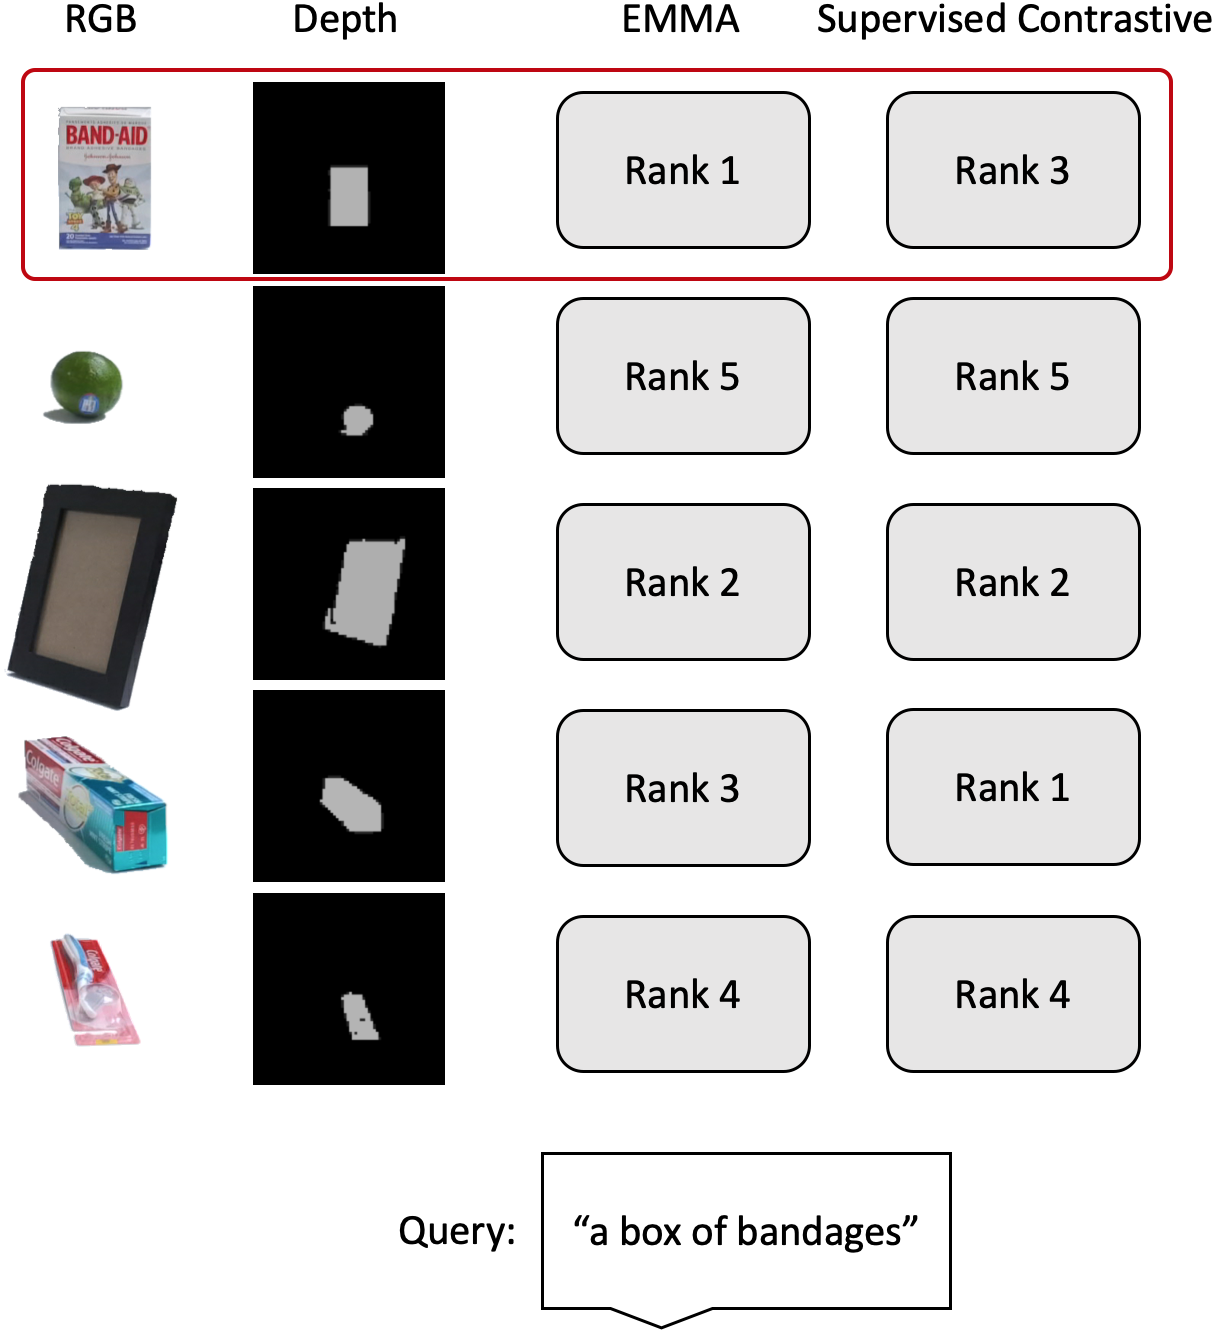
\includegraphics[width=.8\columnwidth]{Figures/example-rankings.png}
\caption{EMMA more accurately ranks objects and handles ambiguities with respect to a retrieval query.}
\label{fig:rankings}
\end{figure}

An example of the need to consider multiple modalities jointly is shown in \cref{fig:rankings}, showing how EMMA is able to correctly select an object instance from several similarly shaped and describable objects. 

%===================================================================


\section{Conclusion}
\label{sec:conclusion}

In this work, we have demonstrated the effectiveness of a novel approach to learning from high-dimensional multimodal information. Our approach performs well on an object retrieval task from a testbed that contains four separate modalities, consistent with information that might be available to a physical agent, and outperforms state of the art contrastive learning approaches when one or more modalities is unavailable at test time. Our proposed method is general enough to be applied to a variety of multimodal retrieval problems, and is not limited to purely language-based image retrieval. 

In future, this work will be extended to solve less clearly delineated problems; for example, differentiating among members of a class, as well as across classes. However, this work represents a significant step towards handling such retrieval problems, while not arbitrarily limiting the number of sensor and other modalities that can be incorporated. 

% Another future work is to improve the speech modality so it can contribute more to the training. Right now when text modality is dropped, the performance decreases by about 0.12. Ideally a better model should have the same performance in case of dropout when it is trained using all modalities.

%===================================================================


% ***************** The END of the paper *****************

% %% The acknowledgments section is defined using the "acks" environment
% %% (and NOT an unnumbered section). This ensures the proper
% %% identification of the section in the article metadata, and the
% %% consistent spelling of the heading.
\begin{acks}
To Robert, for the bagels and explaining CMYK and color spaces.
\end{acks}
% \section*{Acknowledgments}



\clearpage
\clearpage
% %%
% %% The next two lines define the bibliography style to be used, and
% %% the bibliography file.
\bibliographystyle{ACM-Reference-Format}
\bibliography{ref}

% %%
% %% If your work has an appendix, this is the place to put it.
\appendix
\label{sec:appendix}


\end{document}

